%
% This is an example LaTeX file which uses the SANDreport class file.
% It shows how a SAND report should be formatted, what sections and
% elements it should contain, and how to use the SANDreport class.
% It uses the LaTeX article class, but not the strict option.
% ItINLreport uses .eps logos and files to show how pdflatex can be used
%
% Get the latest version of the class file and more at
%    http://www.cs.sandia.gov/~rolf/SANDreport
%
% This file and the SANDreport.cls file are based on information
% contained in "Guide to Preparing {SAND} Reports", Sand98-0730, edited
% by Tamara K. Locke, and the newer "Guide to Preparing SAND Reports and
% Other Communication Products", SAND2002-2068P.
% Please send corrections and suggestions for improvements to
% Rolf Riesen, Org. 9223, MS 1110, rolf@cs.sandia.gov
%
\documentclass[pdf,12pt]{INLreport}
% pslatex is really old (1994).  It attempts to merge the times and mathptm packages.
% My opinion is that it produces a really bad looking math font.  So why are we using it?
% If you just want to change the text font, you should just \usepackage{times}.
% \usepackage{pslatex}
\usepackage{times}
\usepackage[FIGBOTCAP,normal,bf,tight]{subfigure}
\usepackage{amsmath}
\usepackage{amssymb}
\usepackage{soul}
\usepackage{pifont}
\usepackage{enumerate}
\usepackage{listings}
\usepackage{fullpage}
\usepackage{xcolor}          % Using xcolor for more robust color specification
\usepackage{ifthen}          % For simple checking in newcommand blocks
\usepackage{textcomp}
\usepackage{mathtools}
\usepackage{relsize}
\usepackage{lscape}
\usepackage[toc,page]{appendix}
\usepackage{RAVEN}

\newtheorem{mydef}{Definition}
\newcommand{\norm}[1]{\lVert#1\rVert}
%\usepackage[table,xcdraw]{xcolor}
%\usepackage{authblk}         % For making the author list look prettier
%\renewcommand\Authsep{,~\,}

% Custom colors
\definecolor{deepblue}{rgb}{0,0,0.5}
\definecolor{deepred}{rgb}{0.6,0,0}
\definecolor{deepgreen}{rgb}{0,0.5,0}
\definecolor{forestgreen}{RGB}{34,139,34}
\definecolor{orangered}{RGB}{239,134,64}
\definecolor{darkblue}{rgb}{0.0,0.0,0.6}
\definecolor{gray}{rgb}{0.4,0.4,0.4}

\lstset {
  basicstyle=\ttfamily,
  frame=single
}


\setcounter{secnumdepth}{5}
\lstdefinestyle{XML} {
    language=XML,
    extendedchars=true,
    breaklines=true,
    breakatwhitespace=true,
%    emph={name,dim,interactive,overwrite},
    emphstyle=\color{red},
    basicstyle=\ttfamily,
%    columns=fullflexible,
    commentstyle=\color{gray}\upshape,
    morestring=[b]",
    morecomment=[s]{<?}{?>},
    morecomment=[s][\color{forestgreen}]{<!--}{-->},
    keywordstyle=\color{cyan},
    stringstyle=\ttfamily\color{black},
    tagstyle=\color{darkblue}\bf\ttfamily,
    morekeywords={name,type},
%    morekeywords={name,attribute,source,variables,version,type,release,x,z,y,xlabel,ylabel,how,text,param1,param2,color,label},
}
\lstset{language=python,upquote=true}

\usepackage{titlesec}
\newcommand{\sectionbreak}{\clearpage}
\setcounter{secnumdepth}{4}

%\titleformat{\paragraph}
%{\normalfont\normalsize\bfseries}{\theparagraph}{1em}{}
%\titlespacing*{\paragraph}
%{0pt}{3.25ex plus 1ex minus .2ex}{1.5ex plus .2ex}

%%%%%%%% Begin comands definition to input python code into document
\usepackage[utf8]{inputenc}

% Default fixed font does not support bold face
\DeclareFixedFont{\ttb}{T1}{txtt}{bx}{n}{9} % for bold
\DeclareFixedFont{\ttm}{T1}{txtt}{m}{n}{9}  % for normal

\usepackage{listings}

% Python style for highlighting
\newcommand\pythonstyle{\lstset{
language=Python,
basicstyle=\ttm,
otherkeywords={self, none, return},             % Add keywords here
keywordstyle=\ttb\color{deepblue},
emph={MyClass,__init__},          % Custom highlighting
emphstyle=\ttb\color{deepred},    % Custom highlighting style
stringstyle=\color{deepgreen},
frame=tb,                         % Any extra options here
showstringspaces=false            %
}}


% Python environment
\lstnewenvironment{python}[1][]
{
\pythonstyle
\lstset{#1}
}
{}

% Python for external files
\newcommand\pythonexternal[2][]{{
\pythonstyle
\lstinputlisting[#1]{#2}}}

\lstnewenvironment{xml}
{}
{}

% Python for inline
\newcommand\pythoninline[1]{{\pythonstyle\lstinline!#1!}}

% Named Colors for the comments below (Attempted to match git symbol colors)
\definecolor{RScolor}{HTML}{8EB361}  % Sonat (adjusted for clarity)
\definecolor{DPMcolor}{HTML}{E28B8D} % Dan
\definecolor{JCcolor}{HTML}{82A8D9}  % Josh (adjusted for clarity)
\definecolor{AAcolor}{HTML}{8D7F44}  % Andrea
\definecolor{CRcolor}{HTML}{AC39CE}  % Cristian
\definecolor{RKcolor}{HTML}{3ECC8D}  % Bob (adjusted for clarity)
\definecolor{DMcolor}{HTML}{276605}  % Diego (adjusted for clarity)
\definecolor{PTcolor}{HTML}{990000}  % Paul

\def\DRAFT{} % Uncomment this if you want to see the notes people have been adding
% Comment command for developers (Should only be used under active development)
\ifdefined\DRAFT
  \newcommand{\nameLabeler}[3]{\textcolor{#2}{[[#1: #3]]}}
\else
  \newcommand{\nameLabeler}[3]{}
\fi
\newcommand{\alfoa}[1] {\nameLabeler{Andrea}{AAcolor}{#1}}
\newcommand{\cristr}[1] {\nameLabeler{Cristian}{CRcolor}{#1}}
\newcommand{\mandd}[1] {\nameLabeler{Diego}{DMcolor}{#1}}
\newcommand{\maljdan}[1] {\nameLabeler{Dan}{DPMcolor}{#1}}
\newcommand{\cogljj}[1] {\nameLabeler{Josh}{JCcolor}{#1}}
\newcommand{\bobk}[1] {\nameLabeler{Bob}{RKcolor}{#1}}
\newcommand{\senrs}[1] {\nameLabeler{Sonat}{RScolor}{#1}}
\newcommand{\talbpaul}[1] {\nameLabeler{Paul}{PTcolor}{#1}}
% Commands for making the LaTeX a bit more uniform and cleaner
\newcommand{\TODO}[1]    {\textcolor{red}{\textit{(#1)}}}
\newcommand{\xmlAttrRequired}[1] {\textcolor{red}{\textbf{\texttt{#1}}}}
\newcommand{\xmlAttr}[1] {\textcolor{cyan}{\textbf{\texttt{#1}}}}
\newcommand{\xmlNodeRequired}[1] {\textcolor{deepblue}{\textbf{\texttt{<#1>}}}}
\newcommand{\xmlNode}[1] {\textcolor{darkblue}{\textbf{\texttt{<#1>}}}}
\newcommand{\xmlString}[1] {\textcolor{black}{\textbf{\texttt{'#1'}}}}
\newcommand{\xmlDesc}[1] {\textbf{\textit{#1}}} % Maybe a misnomer, but I am
                                                % using this to detail the data
                                                % type and necessity of an XML
                                                % node or attribute,
                                                % xmlDesc = XML description
\newcommand{\default}[1]{~\\*\textit{Default: #1}}
\newcommand{\nb} {\textcolor{deepgreen}{\textbf{~Note:}}~}


%%%%%%%% End comands definition to input python code into document

%\usepackage[dvips,light,first,bottomafter]{draftcopy}
%\draftcopyName{Sample, contains no OUO}{70}
%\draftcopyName{Draft}{300}

% The bm package provides \bm for bold math fonts.  Apparently
% \boldsymbol, which I used to always use, is now considered
% obsolete.  Also, \boldsymbol doesn't even seem to work with
% the fonts used in this particular document...
\usepackage{bm}


% Define tensors to be in bold math font.
\newcommand{\tensor}[1]{{\bm{#1}}}

% Override the formatting used by \vec.  Instead of a little arrow
% over the letter, this creates a bold character.
\renewcommand{\vec}{\bm}

% Define unit vector notation.  If you don't override the
% behavior of \vec, you probably want to use the second one.
\newcommand{\unit}[1]{\hat{\bm{#1}}}
% \newcommand{\unit}[1]{\hat{#1}}

% Use this to refer to a single component of a unit vector.
\newcommand{\scalarunit}[1]{\hat{#1}}

% \toprule, \midrule, \bottomrule for tables
\usepackage{booktabs}

% \llbracket, \rrbracket
\usepackage{stmaryrd}

\usepackage{hyperref}
\hypersetup{
    colorlinks,
    citecolor=black,
    filecolor=black,
    linkcolor=black,
    urlcolor=black
}

% Compress lists of citations like [33,34,35,36,37] to [33-37]
\usepackage{cite}

% If you want to relax some of the SAND98-0730 requirements, use the "relax"
% option. It adds spaces and boldface in the table of contents, and does not
% force the page layout sizes.
% e.g. \documentclass[relax,12pt]{SANDreport}
%
% You can also use the "strict" option, which applies even more of the
% SAND98-0730 guidelines. It gets rid of section numbers which are often
% useful; e.g. \documentclass[strict]{SANDreport}

% The INLreport class uses \flushbottom formatting by default (since
% it's intended to be two-sided document).  \flushbottom causes
% additional space to be inserted both before and after paragraphs so
% that no matter how much text is actually available, it fills up the
% page from top to bottom.  My feeling is that \raggedbottom looks much
% better, primarily because most people will view the report
% electronically and not in a two-sided printed format where some argue
% \raggedbottom looks worse.  If we really want to have the original
% behavior, we can comment out this line...
\raggedbottom
\setcounter{secnumdepth}{5} % show 5 levels of subsection
\setcounter{tocdepth}{5} % include 5 levels of subsection in table of contents

% ---------------------------------------------------------------------------- %
%
% Set the title, author, and date
%
\title{RAVEN Theory Manual and User Guide}
%\author{%
%\begin{tabular}{c} Author 1 \\ University1 \\ Mail1 \\ \\
%Author 3 \\ University3 \\ Mail3 \end{tabular} \and
%\begin{tabular}{c} Author 2 \\ University2 \\ Mail2 \\ \\
%Author 4 \\ University4 \\ Mail4\\
%\end{tabular} }


\author{
\\Andrea Alfonsi
\\Cristian Rabiti
\\Diego Mandelli
\\Joshua Cogliati
\\Congjian Wang
\\Paul W. Talbot
\\Daniel P. Maljovec
\\Curtis Smith
}
% \\James B. Tompkins}   Just people who actually ``developed'' a significant capability in the code should be placed here. Andrea
%\author{\textbf{\textit{Main Developers:}}  \\Andrea Alfonsi}
%\affil{Idaho National Laboratory, Idaho Falls, ID 83402}
%\\\{cristian.rabiti, andrea.alfonsi, joshua.cogliati, diego.mandelli, robert.kinoshita, ramazan.sen\}@inl.gov}

% There is a "Printed" date on the title page of a SAND report, so
% the generic \date should [WorkingDir:]generally be empty.
\date{}


% ---------------------------------------------------------------------------- %
% Set some things we need for SAND reports. These are mandatory
%
\SANDnum{INL/EXT-16-38178}
\SANDprintDate{March 2017}
\SANDauthor{Andrea Alfonsi, Cristian Rabiti, Diego Mandelli, Joshua Cogliati, Congjian Wang, Paul W. Talbot, Daniel P. Maljovec, Curtis Smith}
\SANDreleaseType{Revision 1 draft}


% ---------------------------------------------------------------------------- %
% Include the markings required for your SAND report. The default is "Unlimited
% Release". You may have to edit the file included here, or create your own
% (see the examples provided).
%
% \include{MarkOUO} % Not needed for unlimted release reports

\def\component#1{\texttt{#1}}

% ---------------------------------------------------------------------------- %
\newcommand{\systemtau}{\tensor{\tau}_{\!\text{SUPG}}}

% Added by Sonat
\usepackage{placeins}
\usepackage{array}

\newcolumntype{L}[1]{>{\raggedright\let\newline\\\arraybackslash\hspace{0pt}}m{#1}}
\newcolumntype{C}[1]{>{\centering\let\newline\\\arraybackslash\hspace{0pt}}m{#1}}
\newcolumntype{R}[1]{>{\raggedleft\let\newline\\\arraybackslash\hspace{0pt}}m{#1}}

% end added by Sonat
% ---------------------------------------------------------------------------- %
%
% Start the document
%

\begin{document}

    \maketitle

    % ------------------------------------------------------------------------ %
    % An Abstract is required for SAND reports
    %
%    \begin{abstract}
%    \input abstract
%    \end{abstract}


    % ------------------------------------------------------------------------ %
    % An Acknowledgement section is optional but important, if someone made
    % contributions or helped beyond the normal part of a work assignment.
    % Use \section* since we don't want it in the table of context
    %
%    \clearpage
%    \section*{Acknowledgment}



%	The format of this report is based on information found
%	in~\cite{Sand98-0730}.


    % ------------------------------------------------------------------------ %
    % The table of contents and list of figures and tables
    % Comment out \listoffigures and \listoftables if there are no
    % figures or tables. Make sure this starts on an odd numbered page
    %
    \cleardoublepage		% TOC needs to start on an odd page
    \tableofcontents
    %\listoffigures
    %\listoftables


    % ---------------------------------------------------------------------- %
    % An optional preface or Foreword
%    \clearpage
%    \section*{Preface}
%    \addcontentsline{toc}{section}{Preface}
%	Although muggles usually have only limited experience with
%	magic, and many even dispute its existence, it is worthwhile
%	to be open minded and explore the possibilities.


    % ---------------------------------------------------------------------- %
    % An optional executive summary
    %\clearpage
    %\section*{Summary}
    %\addcontentsline{toc}{section}{Summary}
    %\input{Summary.tex}
%	Once a certain level of mistrust and skepticism has
%	been overcome, magic finds many uses in todays science



%	and engineering. In this report we explain some of the
%	fundamental spells and instruments of magic and wizardry. We
%	then conclude with a few examples on how they can be used
%	in daily activities at national Laboratories.


    % ---------------------------------------------------------------------- %
    % An optional glossary. We don't want it to be numbered
%    \clearpage
%    \section*{Nomenclature}
%    \addcontentsline{toc}{section}{Nomenclature}
%    \begin{description}
%          \item[alohomoral]
%           spell to open locked doors and containers
%          \item[leviosa]
%           spell to levitate objects
%    \item[remembrall]
%           device to alert you that you have forgotten something
%    \item[wand]
%           device to execute spells
%    \end{description}


    % ---------------------------------------------------------------------- %
    % This is where the body of the report begins; usually with an Introduction
    %
    \SANDmain		% Start the main part of the report

\section{Introduction}
\label{sec:introduction}
RAVEN (\textbf{R}isk \textbf{A}nalysis \textbf{V}irtual \textbf{EN}vironment)~\cite{Nureg1150}  is one of the many INL-developed software tools researchers can 
use to identify and 
increase the safety margin in complex systems (e.g. Nuclear Power Plants). It is a modular or ``plug-able'' framework that can be coupled with other computer 
modeling systems. RAVEN is capable to agnostically communicate with any system 
code. This agnosticism includes providing Application Programming Interfaces (APIs). These APIs are used to allow RAVEN to interact with any code as long as all 
the parameters that need to be perturbed are accessible through input files or via python interfaces. 
As a generic software framework, RAVEN is designed to perform parametric and probabilistic analysis based on the response of complex system codes. RAVEN is 
capable of investigating the system response as well as the input space using standard sampling techniques (e.g Monte Carlo, Grid, or Latin Hyper Cube), but its 
strength is focused toward system feature discovery, such as limit surfaces (i.e. separating regions of the input space leading to system failure, using dynamic 
supervised learning techniques), and advanced data analysis methodologies (i.e. Topology-based domain decomposition, Data Mining, Clustering, etc.).

The development of RAVEN has begun in 2012 to satisfy the need to provide a modern risk evaluation framework. RAVEN principal assignment is to provide the 
necessary software and algorithms in order to employ the concept developed by the Risk Informed Safety Margin Characterization (RISMC) path-
way~\cite{RISMC}. 
RISMC is one of the pathways defined within the Light Water Reactor Sustainability (LWRS) program. In the RISMC approach, the goal is not just specifically 
identifying the frequency of an event potentially leading to a system failure, but also to analyze the ``distance'' and the drivers toward the happening of key 
safety-related events. This approach may be used in identifying and increasing the safety margins related to those events. A safety margin is a numerical value 
quantifying the probability that a safety metric (e.g. as peak pressure in a pipe) is exceeded under certain conditions. The initial development of RAVEN has 
been focused on providing dynamic risk assessment capability to RELAP-7~\cite{RELAP7}, currently under development at the INL. All the methodologies
developed have been modularized in order to be applied to any computer modeling system (e.g., BISON, RELAP-7, RELAP5-3D, MELCOR, etc.).

The aim of this manuscript is to present a peculiar capability within the RAVEN framework named \textit{``EnsembleModels''}.

RAVEN is currently able to construct multi-targets Reduced Order Models (Ref.4), which are aimed to represent the response of a system (in a 
fixed configuration) for multiple Figures of Merits (FOMs) and time-dependent ROMs (see Ref.5). These capabilities represent the initial steps for a larger 
implementation about the interaction of multiple models. In fact, in several cases, multiple models need to interface with each other since the initial conditions of 
one are dependent on the outcomes of another.
To better understand the problem that here is solved, it is useful to consider two simple examples:
\begin{enumerate}
  \item The following problem is considered: a weather forecast simulation code ``a'' is used to compute the external (i.e. ambient) temperature in a certain location. 
  A second model ``b'' is inquired to compute the average temperature in a room having as boundary condition, among several others, the external ambient 
  temperature. The response of the model ``b'' depends on the outcome of the model ``a'';
   \item Two different simulation codes are considered: a) a code that is meant to compute the thermal conductivity of the ceramic Uranium Dioxide (UO2) as 
   function of the Temperature, and b) a Thermal-hydraulic (TH) code that is used to compute the Temperature field of a reactor, whose heat conduction depends on 
   the thermal conductivity value. As easily inferable, the two models are mutual dependent, determining in a non-linear system of equations.
\end{enumerate}
The two reported examples are only aimed to illustrate the reason why the creation of a framework to make interact different models is a key development for the 
advancement of RAVEN as a comprehensive calculation flow driver. Before reporting how the ensemble-models have been implemented, it is necessary to briefly 
describe the representative Model ``entities'' that are available in RAVEN.



\begin{figure}
    \centering
    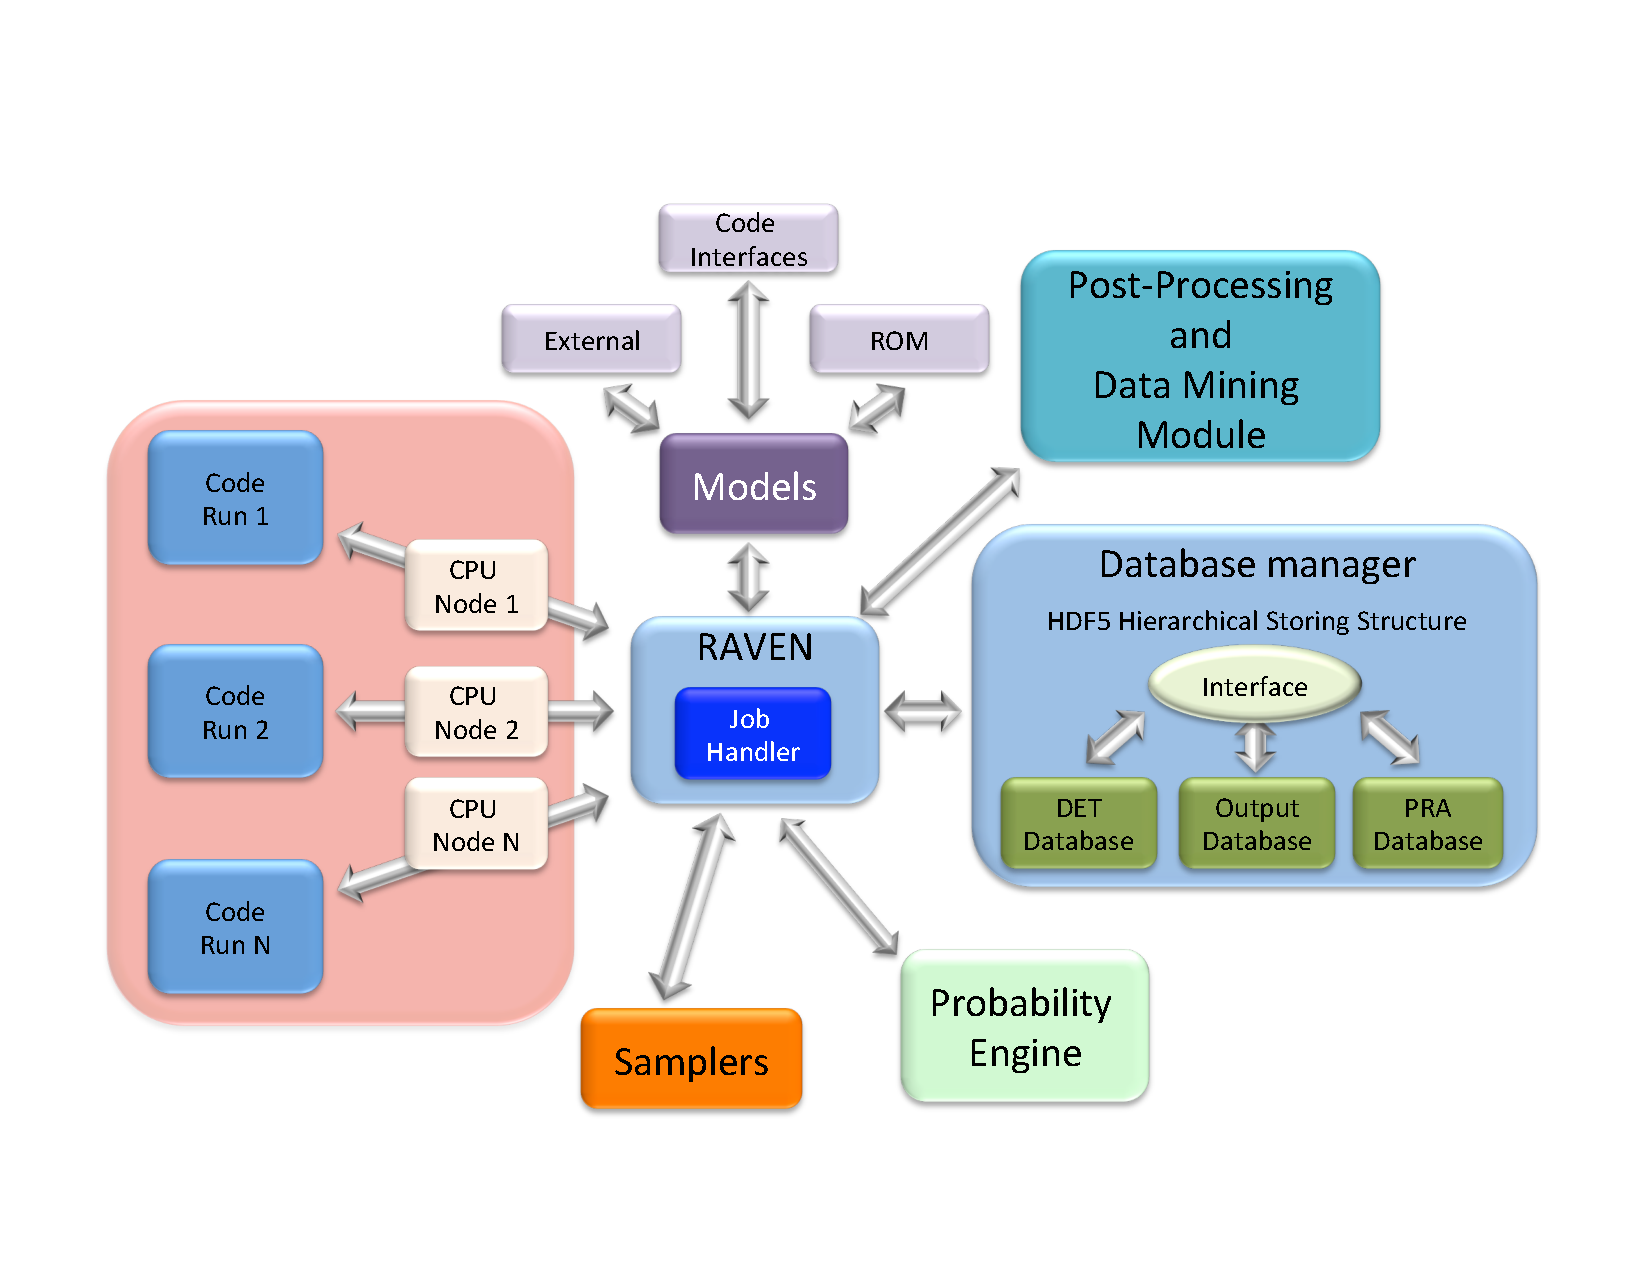
\includegraphics[scale=0.5]{raven.pdf}
    \caption{RAVEN}
    \label{fig:raven}
\end{figure}

\section{RAVEN Concepts}
\label{sec:RAVENconcept}
After the brief overview of the RAVEN code, it is necessary to focus on the main concepts that are behind the design of the framework:
\begin{itemize}
    \item \textit{RAVEN entities}: Section ~\ref{sub:EntitiesAndFlow} is aimed to provide an overview on how the different objects in
    RAVEN can interact with each other, generating the user-dependent analysis flow
    \item \textit{RAVEN input main components}: Section ~\ref{sub:InputStructure} provides a brief introduction of the input structure, introducing
    some of the input ``structure'' that are going to be used in this manual. A detailed explanation of the
    input structure and keywords is reported in the user manual ~\cite{RAVENuserManual}.
\end{itemize}
\subsection{RAVEN Entities and Analysis Flow}
\label{sub:EntitiesAndFlow}
In the RAVEN code the number and types of possible analyses is potentially large (it is customization to many problem types).
\\Each basic action (sampling, printing, etc.) is encapsulated in
a dedicated object (named ``\textbf{Entity}''). Each object is inactive till it is connected with
other objects in order to perform a more complex process. For example,
the \textit{Sampler} entity, aimed to employ a perturbation action, becomes active only in case
it gets associated with a \textit{Model}, that is the internal representation of a physical model (e.g.,a system code).
\\RAVEN provides support for several \textbf{Entities}, which branch in several different categories/algorithms:
\begin{itemize}
  \item \textit{\textbf{RunInfo}}:
    \\The RunInfo \textbf{Entity} is an information container which describes how the overall computation should
      be performed. This \textbf{Entity}  accepts several input settings that define how to drive the calculation and set up,
      when needed, particular settings for the machine the code needs to run on (queue system, if not Portable Batch System-PBS, etc.).
  \item \textit{\textbf{Files}}:
  \\ The Files \textbf{Entity}  defines any files that might be needed within the RAVEN run. This could include inputs to the
      Model, pickled ROM files, or Comma Separated Value (CSV) files for post-processors, to name a few.
  \item \textit{\textbf{DataObjects}}:
    \\The DataObjects system is a container of data objects of various types that can be constructed during the execution of
    desired calculation flow. These data objects can be used as input or output for a particular \textit{Model}
     \textbf{Entity}. Currently RAVEN supports four different data types, each with a particular conceptual meaning:
     \begin{itemize}
        \item \textit{Point} describes the state of the system at a certain point (e.g.,in time). In other words, it can be
                                       considered a mapping between a set of parameters in the input space and the resulting
                                       outcomes in the output space at a particular point in the phase space (e.g.,in time).
        \item \textit{PointSet} is a collection of individual Point objects. It can be considered a mapping between multiple
                                            sets of parameters in the input space and the resulting sets of outcomes in the output space
                                            at a particular point (e.g., in time).
        \item \textit{History} describes the temporal evolution of the state of the system within a certain input domain;
        \item \textit{HistorySet} is a collection of individual History objects. It can be considered a mapping between
                                               multiple sets of parameters in the input space and the resulting sets of temporal evolution
                                               in the output space.
     \end{itemize}
     The DataObjects represent the preferred way to transfer the information coming from a Model (e.g., the driven code) to
      all the other RAVEN systems (e.g., Out-Stream system, Reduced Order Modeling component, etc.).
  \item \textit{\textbf{Databases}}:
      \\ RAVEN provides the capability to store and retrieve data to/from an external database. Currently RAVEN supports
       only a database type called \textit{HDF5}. This database, depending on the data format it is receiving, will
       organize itself in a ``parallel'' or ``hierarchical'' fashion. The user can create as many database \textbf{Entities} as needed.
  \item \textit{\textbf{Samplers}}:
  \\ The Samplers  \textbf{Entity} is the container of all the algorithms designed to perform the perturbation of the input space.
      The Samplers can be categorized into three main classes:
      \begin{itemize}
        \item  \textit{Forward}. Sampling strategies that do not leverage the information coming from already evaluated
        realizations in the input space. For example, Monte-Carlo, Stratified (LHS), Grid, Response Surface, Factorial Design,
        Sparse Grid, etc.
        \item  \textit{Adaptive}. Sampling strategies that take advantages of the information coming from already evaluated
        realizations of the input space, adapting the sampling strategies to key figures of merits. For example, Limit Surface
        search, Adaptive HDMR, etc.
        \item \textit{Dynamic Event Tree}. Sampling strategies that perform the exploration of the input space based on the
        dynamic evolution of the system, employing branching techniques. For example, Dynamic Event Tree, Hybrid
        Dynamic Event Tree, etc.
      \end{itemize}
  \item \textit{\textbf{OutStreams}}:
  \\ The OutStreams node is the \textbf{Entity} used for data exporting and dumping. The OutStreams support
   2 actions:
      \begin{itemize}
       \item \textit{Print}. This Out-Stream is able to print out (in a Comma Separated Value format) all the information
         contained in:
         \begin{itemize}
          \item DataObjects
          \item Reduced Order Models.
         \end{itemize}
       \item \textit{Plot}. This Out-Stream is able to plot 2-Dimensional, 3-Dimensional, 4-Dimensional (using color
       mapping) and 5-Dimensional (using marker size). Several types of plot are available, such as scatter, line, surfaces,
       histograms, pseudo-colors, contours, etc.
      \end{itemize}
  \item \textit{\textbf{Distributions}}:
  \\ The Distributions \textbf{Entity} is the container of all the stochastic representations of random variables. Currently,
  RAVEN supports:
      \begin{itemize}
       \item \textit{1-Dimensional} continuous and discrete distributions, such as Normal, Weibull, Binomial, etc.
       \item \textit{N-Dimensional} distributions, such as Multivariate Normal, user-inputted N-Dimensional distributions.
      \end{itemize}
\begin{figure}[h!]
  \includegraphics[scale=1]{pics/ExampleStepEntity.png}
  \caption{Example of the Steps \textbf{Entity}  and its connection in the input file.}
  \label{fig:ExampleStepEntity}
\end{figure}
  \item \textit{\textbf{Models}}:
  \\ The Models \textbf{Entity}  represents the projection from the input to the output space. Currently, RAVEN defines the
  following sub-categories:
      \begin{itemize}
       \item \textit{Code}, the sub-~\textbf{Entity} that represent the driven code, through external code interfaces (see~\cite{RAVENuserManual})
       \item  \textit{ExternalModel}, the sub-~\textbf{Entity} that represents a physical or mathematical model that is
       directly implemented by the user in a Python module
      \item \textit{ROM}, the sub-~\textbf{Entity} that represent the Reduced Order Model, interfaced with several algorithms
       \item \textit{PostProcessor}, the sub-~\textbf{Entity} that is used to perform action on data, such as computation of
       statistical moments, correlation matrices, etc.
      \end{itemize}
      The Model \textbf{Entity} can be seen as a transfer function between the input and output space.
  \item \textit{\textbf{Functions}}:
   \\ The Functions \textbf{Entity} is the container of all the user-defined functions, such as Goal Functions in adaptive
   sampling strategies, etc.
\end{itemize}
All these action-objects are combined together to create a peculiar analysis flow, which is specified
by the user in an additional \textbf{Entity} named \textit{\textbf{Steps}}. This \textbf{Entity} represents the core of the analysis, since it is the location where the multiple objects get finally linked in order to perform a combined action on a certain \textit{Model} (see Fig.~\ref{fig:ExampleStepEntity}). In order to perform this linking, each \textbf{Entity} defined in the Step needs to ``play'' a Role:
\begin{itemize}
  \item \textit{Input}
  \item \textit{Output}
  \item \textit{Model}
  \item \textit{Sampler}
  \item \textit{Function}
  \item \textit{ROM}
  \item \textit{SolutionExport}, the \textbf{Entity} that is used to export the solution of a \textit{Sampler}.
\end{itemize}
Currently, RAVEN supports 4 different types of \textit{\textbf{Steps}}:
\begin{itemize}
  \item \textit{SingleRun}, perform a single run of a model
  \item \textit{MultiRun}, perform multiple runs of a model
  \item \textit{RomTrainer}, perform the training of a Reduced Order Model (ROM)
  \item \textit{PostProcess}, post-process data or manipulate RAVEN entities
  \item \textit{IOStep}, step aimed to perform multiple actions:
  \begin{itemize}
    \item construct/update a Database from a DataObjects and vice-versa
    \item construct/update a Database or a DataObjects object from CSV files
    \item stream the content of a Database or a DataObjects out through an OutStream
    \item store/retrieve a ROM to/from an external File using Pickle module of Python
  \end{itemize}
\end{itemize}

\subsection{Raven Input Structure}
\label{sub:InputStructure}
The RAVEN code does not have a fixed calculation flow, since all of its basic
objects can be combined in order to create a user-defined calculation flow.
%
Thus, its input, eXtensible Markup Language (XML) format, is organized in different XML blocks, each with a
different functionality.
%
The main input blocks are as follows:
\begin{itemize}
  \item \textbf{\textless Simulation\textgreater}: The root node containing the
  entire input, all of
  the following blocks fit inside the \emph{Simulation} block.
  %
  \item \textbf{\textless RunInfo\textgreater}: Specifies the calculation
  settings (number of parallel simulations, etc.).
  %
  \item \textbf{\textless Files\textgreater}: Specifies the files to be
  used in the calculation.
  %
  \item \textbf{\textless Distributions\textgreater}: Defines distributions
  needed for describing parameters, etc.
  %
  \item \textbf{\textless Samplers\textgreater}: Sets up the strategies used for
  exploring an uncertain domain.
  %
  \item \textbf{\textless DataObjects\textgreater}: Specifies internal data objects
  used by RAVEN.
  %
  \item \textbf{\textless Databases\textgreater}: Lists the HDF5 databases used
  as input/output to a
  RAVEN run.
  %
  \item \textbf{\textless OutStreams\textgreater}: Visualization and
  Printing system block.
  %
  \item \textbf{\textless Models\textgreater}: Specifies codes, ROMs,
  post-processing analysis, etc.
  %
  \item \textbf{\textless Functions\textgreater}: Details interfaces to external
  user-defined functions and modules.
  %
  the user will be building and/or running.
  %
  \item \textbf{\textless Steps\textgreater}: Combines other blocks to detail a
  step in the RAVEN workflow including I/O and computations to be performed.
  %
\end{itemize}

Each of these blocks are explained in dedicated sections of the user manual ~\cite{RAVENuserManual}.
%

\section{Forward Sampling Strategies}
\label{sec:forwardSamplingStrategies}
In order to perform UQ and dynamic
probabilistic risk assessment (DPRA),
a sampling strategy needs to be employed. The sampling strategy
perturbs the input space (domain of the uncertainties) to explore
the response of a complex system in relation to selected figure of merits (FOMs).

The most widely used strategies to perform UQ and PRA are generally
collected in RAVEN as \textit{\textbf{Forward}} samplers. \textit{\textbf{Forward}} samplers include
all the strategies that simply perform the sampling of the input space.  These strategies sample
without exploiting, through learning approaches,
the information made available from the outcomes of evaluation previously performed (adaptive sampling) and the
common system evolution (patterns) that different sampled calculations can generate in the phase space (Dynamic Event Tree).

RAVEN has several different \textit{\textbf{Forward}} samplers:
\begin{itemize}
  \item \textit{Monte-Carlo}
  \item \textit{Grid-based}
  \item \textit{Stratified} and its specialization named \textit{Latin Hyper Cube}.
\end{itemize}
In addition, RAVEN posses advanced \textit{\textbf{Forward}} sampling strategies that:
\begin{itemize}
  \item Build a grid in the input space selecting evaluation points
    based on characteristic quadratures as part of stochastic collocation
    for generalized polynomial chaos method (\textit{Sparse
    Grid Collocation} sampler);
  \item Use high-density model reduction (HDMR) a.k.a. Sobol
    decomposition to approximate a function as the sum of
    interactions with increasing complexity (\textit{Sobol} sampler).
\end{itemize}
In the following subsections, the theory behind these sampling
methodologies is explained.
%%%%%%%%%%%%%%%%%%%%%%%%%
%%%%%%%%  MONTE-CARLO %%%%%%%%
%%%%%%%%%%%%%%%%%%%%%%%%%
\subsection{Monte-Carlo}
\label{sub:MC}
The Monte-Carlo method is one of the most-used methodologies in several mathematic disciplines.
It approximates an expectation by the sample mean of a function of
simulated random variables. It is based on the laws of large numbers in order to approximate expectations.
In order words, it approximates the average response of multiple FOMs
relying on multiple random sampling of the input space.
\\Consider a random variable (eventually multidimensional) $X$ having probability mass function or probability density function $pdf_{X}(x)$,
which is greater than zero on a set of values $\chi$. Then the expected value of a function $f$ of $X$ is as follows:
\begin{equation}
\begin{matrix}
\mathbb{E}(f(X)) =\sum_{x \in \chi} f(x)pdf_{X}(x) & \text{if} X \, discrete \\
\\
\mathbb{E}(f(X)) =\int_{x \in \chi} f(x)pdf_{X}(x) & \, \text{if} X \, \, continuous
\end{matrix}
\end{equation}
Now consider $n$ samples of $X$, $(x_{1},...,x_{n})$, and compute the mean of $f(x)$ over the samples. This computation represents the Monte-Carlo estimate:
\begin{equation}
  \mathbb{E}(f(X)) \approx   \widetilde{f}_{n}(x) = \frac{1}{n} \sum_{i=1}^{n} f(x_{i})
\end{equation}
If $\mathbb{E}(f(X))$ exists, then the law of large numbers determines that for any arbitrarily small $\varepsilon$:
\begin{equation}
  \lim_{n\rightarrow \, \infty} P( \left | \widetilde{f}_{n}(X) - \mathbb{E}(f(X))  \right |\geq \varepsilon) = 0
\end{equation}
The above equation suggests that as $n$ gets larger, then the probability that $\widetilde{f}_{n}(X)$ deviates
from the $\mathbb{E}(f(X))$ becomes smaller. In other words, the more samples are spooned, the more closer the Monte-Carlo estimate of $X$ gets to the real value.
\\In addition, $\widetilde{f}_{n}(X)$ represent an unbiased estimate for $\mathbb{E}(f(X))$:
\begin{equation}
\mathbb{E}(\widetilde{f}_{n}(X)) = \mathbb{E} \left ( \frac{1}{n} \sum_{i=1}^{n} f(x_{i})   \right ) =
\frac{1}{n} \sum_{i=1}^{n} \mathbb{E}(f(x_{i})) =   \mathbb{E}(f(X))
\end{equation}
%After this brief introduction, it is important to understand how the Monte-Carlo method can be employed
%for the analysis of Dynamic Stochastic system.
%\\Referencing to the nomenclature defined in section~\ref{sub:mathBackground}, given:
%\begin{equation}
%\frac{\partial  \overline{\theta}^{c}\left ( t \right )}{\partial t}=f\left ( \overline{\theta}^{c},\overline{\theta}^{d}_{i}, \overline{\alpha}_{staz} ,\overline{\alpha}_{brow}, t \right )
%\end{equation}
% define a function $g_{i}$ that represents the solution of the previous equation (the trajectory in the $ \overline{\theta}^{c}$ space for a fixed $ \overline{\theta}^{d}_{i}$ and initial condition $\overline{\theta}^{c}_{0}$) :
%\begin{equation}
%  \overline{\theta}^{c}(t) = g_{i}(t,\overline{\theta}^{c}_{0})
%\end{equation}
%The Monte-Carlo analysis is performed as following:
%\begin{enumerate}
%  \item Sample:
%  \begin{itemize}
%    \item $\overline{\alpha}_{staz} $,$\overline{\alpha}_{DS}$, $\overline{t}$ depending on which
%    approximations are valid (see~\ref{sub:mathBackground});
%    \item The initial conditions $\overline{\theta}^{c}_{0}$,$\overline{\theta}^{d}_{0}$;
%    \item Transition conditions from $W(\overline{\theta}^{d}|\overline{\theta}^{d}_{i},\overline{\theta}^{c},t)$
%  \end{itemize}
%  \item Run the system simulator using the previously sampled values and affected by the intrinsic stochasticity
%  represented by $\overline{\alpha}_{brow}$;
%  \item Pause the simulation when a transition condition is reached and move from the current $\overline{\theta}^{d}_{0}$ to the new $\overline{\theta}^{d}$ (e.g. $\overline{\theta}^{d}_{1}$);
%  \item Run the simulation as performed in step 3, starting from the new coordinate and pause the simulation when a new transition is reached;
%  \item Repeat steps 3 and 4 until a stopping condition is reached;
%  \item Repeat 1 through 4 for a large number of runs $n$.
%\end{enumerate}
%%%%%%%%%%%%%%%%%%%%%%%%%
%%%%%%%%          GRID          %%%%%%%%
%%%%%%%%%%%%%%%%%%%%%%%%%
\subsection{Grid}
\label{sub:Grid}
The Grid sampling method (also known as Full Factorial Design of Experiment) represents one of the simplest methodologies that can be employed in order to explore the interaction of multiple random variables with respect
selected FOMs.
The goal of the Grid-based sampling strategy is to explore the interaction of multiple random
variables (i.e.,uncertainties) with respect to selected FOMs. Indeed, this method is mainly used to perform
parametric analysis of the system response rather than a probabilistic one. This method discretizes the
domain of the uncertainties in a user-defined number of intervals (see Figure~\ref{fig:GridDiscretization}) and
record the response of the model (e.g. a system code) at each coordinate (i.e., combination of the uncertainties) of the grid.
\\ This method starts from the assumption that each coordinate on the grid is representative, with respect to the FOMs of interest, of the surrounding grid cell. In other words, it is assumed that the response of a system does not significantly change within the hyper-volume surrounding each grid coordinate (red square in Figure~\ref{fig:GridDiscretization}).
 %%%%%%%%%%%%%%%%%%%%%%%%%%%%%%%%%%%%%%%%%%%%%%%%%%%%%%%%%%
 %figure history
 \begin{figure}[h!]
  \centering
  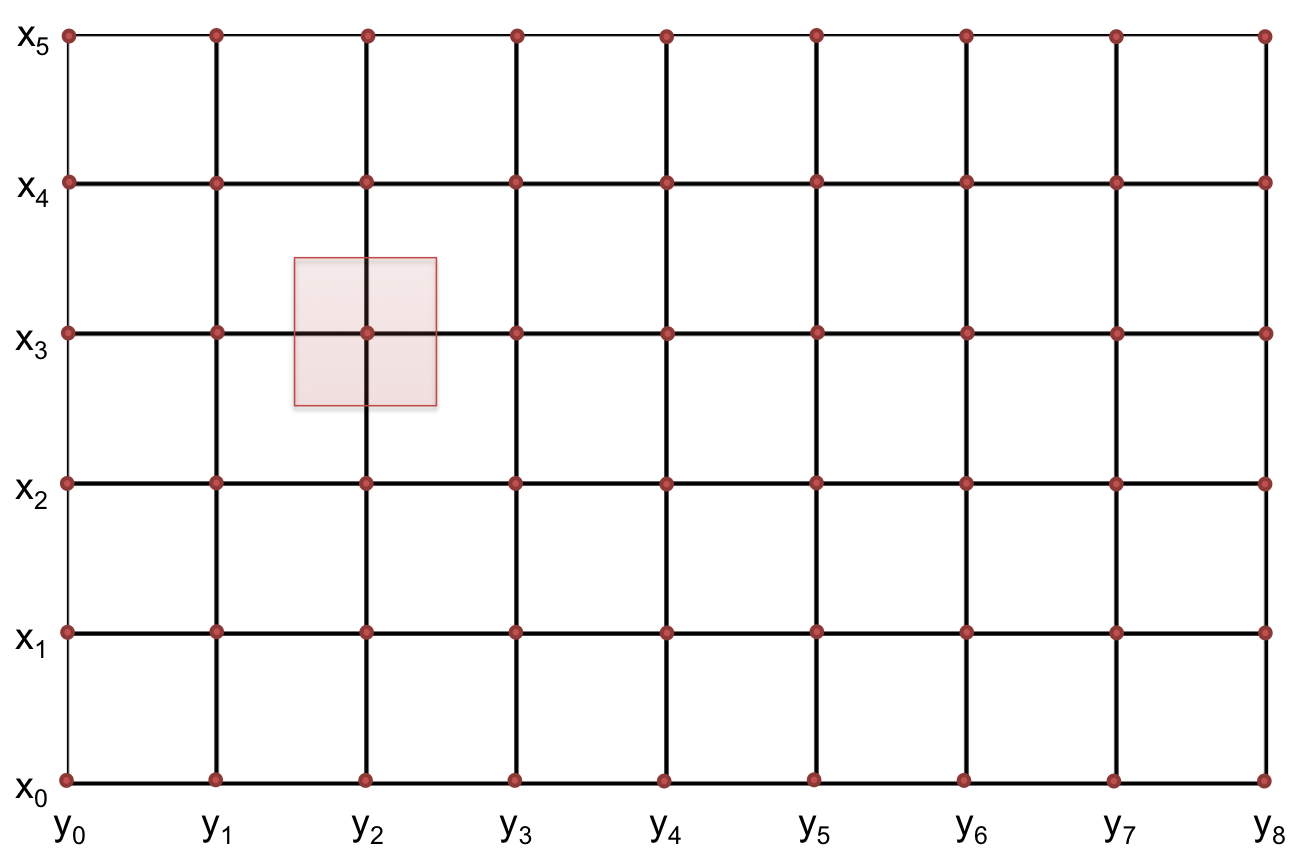
\includegraphics[scale=0.7]{pics/GridDiscretization.png}
  \caption{Example of 2-Dimensional grid discretization. }
  \label{fig:GridDiscretization}
 \end{figure}
 %%%%%%%%%%%%%%%%%%%%%%%%%%%%%%%%%%%%%%%%%%%%%%%%%%%%%%%%%%

Similarly to what has been already reported for the Monte-Carlo sampling, consider a random variable $X$ having PDF $pdf_{X}(x)$ and, consequentially, CDF $cdf_{X}(x)$ in the domain $\chi$. Then the expected value of a function $f$ of $X$ is as follows:
\begin{equation}
\begin{matrix}
\mathbb{E}(f(X)) =\sum_{x \in \chi} f(x)pdf_{X}(x) & if X \, discrete \\
\\
\mathbb{E}(f(X)) =\int_{x \in \chi} f(x)pdf_{X}(x) & \, if X \, \, continuous
\end{matrix}
\end{equation}
In the Grid approach, the domain of $X$ is discretized in a finite number of intervals. Recall that
each node of this discretization is representative of the surrounding hyper-volume. This means that a weight
needs to be associated with each coordinate of the resulting grid:
\begin{equation}
\begin{matrix}
  w_{i}= cdf_{X}(x_{i+1/2}) - cdf_{X}(x_{i-1/2})
\end{matrix}
\end{equation}
Now consider
a $n-$discretization of the domain of  $X$, $(x_{1},...,x_{n})$ and compute the mean of $f(x)$ over the discretization. Based on the previous equation, the computation of the expected value of $f(x)$ is as follows:
\begin{equation}
 \mathbb{E}(f(X)) \approx   \widetilde{f}_{n}(x) = \frac{1}{\sum_{i=1}^{n}w_{i}} \sum_{i=1}^{n} f(x_{i}) \times w_{i}
\end{equation}
If the number of uncertainties under consideration is greater than one ($m$), the above equation
becomes:
\begin{equation}
\mathbb{E}(f(\overline{X})) \approx   \widetilde{f}_{n}(\overline{x}) = \frac{1}{\sum_{i=1}^{n}\prod_{j=1}^{m}w_{i,j}} \sum_{i=1}^{n} f(\overline{x}_{i}) \times \prod_{j=1}^{m}w_{i,j}
\end{equation}
%%%%%%%%%%%%%%%%%%%%%%%%%
%%%%%%%%    STRATIFIED    %%%%%%%%
%%%%%%%%%%%%%%%%%%%%%%%%%
\subsection{Stratified}
\label{sub:Stratified}
The Stratified sampling is a class of methods that relies on the assumption that the input space (i.e.,uncertainties)
can be separated in regions (strata) based on similarity of the response of the system for input set within the
same strata. Following this assumption, the most rewarding (in terms of computational cost vs. knowledge gain)
sampling strategy would be to place one sample for each region. In this way, the same information is not
collected more than once and all the prototypical behavior are sampled at least once. In
Figure~\ref{fig:StratifiedSamplingExample}, the Stratified sampling approach is exemplified.
 \begin{figure}[h!]
  \centering
  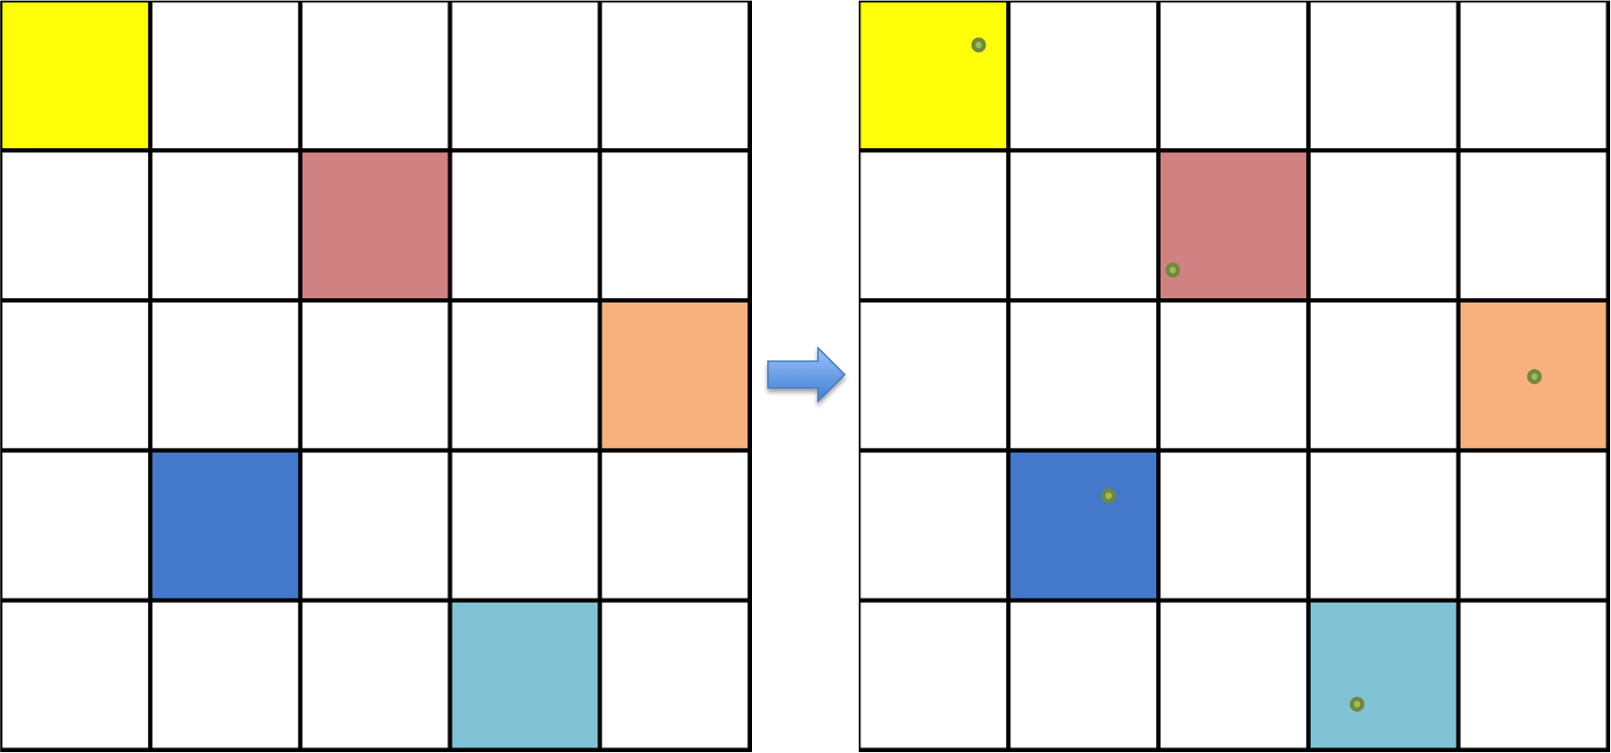
\includegraphics[scale=0.55]{pics/StratifiedSamplingExample.png}
  \caption{Example of Stratified sampling approach.}
  \label{fig:StratifiedSamplingExample}
 \end{figure}
\\The Stratified sampling approach is a method for the exploration of the input space that consists of dividing the uncertain domain into subgroups before sampling. In the Stratified sampling, these subgroups must be:
\begin{itemize}
  \item Mutually exclusive: every element in the population must be assigned to only one stratum (subgroup)
  \item Collectively exhaustive: no population element can be excluded.
\end{itemize}
Then, simple random sampling or systematic sampling is applied within each stratum. The Latin Hyper-Cube sampling represents a specialized version of the stratified approach, when the domain strata are constructed in equally-probable CDF bins.
\\Similarly to what has been already reported for the Grid sampling, consider a set of  $m$ random variables $X_{j}, \, j=1,..,m$ having PDFs $pdf_{X_{j}}(x_{j})$ and, consequentially, CDF $cdf_{X_{j}}(x_{j})$ in the domain $\chi_{j}$. Then the expected value of a function $f$ of $X_{j}, \, j=1,..,m$ is as follows:
\begin{equation}
\begin{matrix}
\mathbb{E}(f(\overline{X})) =\sum f(x)   \prod_{j=1}^{m} pdf_{X_{j}}(x_{j}) & if \overline{X} \, discrete \\
\\
\mathbb{E}(f(\overline{X})) =\int f(x)\prod_{j=1}^{m} pdf_{X_{j}}(x_{j}) & \, if \overline{X} \, \, continuous
\end{matrix}
\end{equation}
In the Stratified approach, the domain of $\overline{X}$ is discretized in a set of strata. Consequentially, similarly to the Grid sampling, a weight needs to be associated with each realization in the input space:
\begin{equation}
\begin{matrix}
  w_{i}= \frac{\prod_{j=1}^{m} \left [  cdf_{X_{j}}(x_{i,j+1}) - cdf_{X_{j}}(x_{i,j}) \right ]}{\sum_{points}\prod_{j=1}^{m} \left [  cdf_{X_{j}}(x_{i,j+1}) - cdf_{X_{j}}(x_{i,j}) \right ]}
\end{matrix}
\end{equation}
Each realization carries a weight representative of each stratum.
\\Now consider
an $n-$strata of the domain of  $\overline{X}$, and compute the expected value of $f(x)$ over the discretization. Based on the previous equation, the computation of the expected value of $f(x)$ is as follows:
\begin{equation}
 \mathbb{E}(f(\overline{X})) \approx   \widetilde{f}_{n}(\overline{x}) = \frac{1}{\sum_{i=1}^{n}w_{i}} \sum_{i=1}^{n} f(\overline{x}_{i}) \times w_{i}
\end{equation}
%%%%%%%%%%%%%%%%%%%%%%%%%
\subsection{Sparse Grid Collocation}
\label{sub:SGC}
The Sparse Grid Collocation sampler represents an advanced methodology to perform Uncertainty Quantification. They aim
to explore the input space leveraging the information contained in the associated probability density functions. It builds on generic Grid sampling by selecting evaluation points based on characteristic quadratures as part of stochastic collocation for generalized polynomial chaos uncertainty quantification. In collocation an N-D grid is constructed, with each uncertain variable providing an axis. Along each axis, the points of evaluation correspond to quadrature points necessary to integrate polynomials. In the simplest (and most naive) case, a N-D tensor product of all possible combinations of points from each dimension’s quadrature is constructed as sampling points. The number of necessary samples can be reduced by employing Smolyak-like sparse grid algorithms, which use reduced combinations of polynomial orders to reduce the necessary sampling space.
\subsubsection{Generalized Polynomial Chaos}
In general, polynomial chaos expansion (PCE) methods seek to interpolate the simulation code as a combination of
polynomials of varying degree in each dimension of the input space.  Originally Wiener
proposed expanding in Hermite polynomials for Gaussian-normal distributed variables~\cite{wiener}.  Askey and
Wilson generalized Hermite polynomials to include Jacobi polynomials, including Legendre and Laguerre
polynomials~\cite{Wiener-Askey}.  Xiu and Karniadakis combines these concepts to perform PCE for a range of Gaussian-based
distributions with corresponding polynomials,
including Legendre polynomials for uniform distributions, Laguerre polynomials for Gamma distributions, and
Jacobi polynomials for Beta distributions \cite{xiu}.

In each of these cases, a probability-weighted
integral over the distribution can be cast in a way that the corresponding polynomials are orthogonal over the
same weight and interval.  These chaos Wiener-Askey polynomials were used by Xiu and Karniadakis to develop
the generalized polynomial chaos expansion method (gPC), including a transformation for applying the same
method to arbitrary distributions (as long as they have a known inverse CDF)~\cite{xiu}.  Two significant
methodologies have grown from gPC application.  The first makes use of Lagrange polynomials to expand the
original function or simulation code, as they can be made orthogonal over the same domain as the
distributions~\cite{SCLagrange}; the other uses the Wiener-Askey polynomials~\cite{xiu}.

Consider a simulation code that produces a quantity of interest $u$ as a function $u(Y)$ whose arguments are
the uncertain, distributed input
parameters $Y=(Y_1,\ldots,Y_n,\ldots,Y_N)$.  A particular realization $\omega$ of $Y_n$ is expressed by
$Y_n(\omega)$, and a single realization of the entire input space results in a solution to the function as
$u(Y(\omega))$. Obtaining a realization of $u(Y)$ may take considerable computation time and
effort.
$u(Y)$ gets expanded in orthonormal multidimensional polynomials $\Phi_k(Y)$, where $k$ is a multi-index tracking
the polynomial order in each axis of the polynomial Hilbert space, and $\Phi_k(Y)$ is constructed as
\begin{equation}\label{eq:gPC}
  \Phi_k(Y) = \prod_{n=1}^N \phi_{k_n}(Y_n),
\end{equation}
where $\phi_{k_n}(Y_n)$ is a single-dimension Wiener-Askey orthonormal polynomial of order $k_n$ and
$k=(k_1,\ldots,k_n,\ldots,k_N)$, $k_n\in\mathbb{N}^0$.  For example, given $u(y_1,y_2,y_3)$, $k=(2,1,4)$
is the multi-index of the
product of a second-order polynomial in $y_1$, a first-order polynomial in $y_2$, and a fourth-order
polynomial in $y_4$. The gPC for $u(Y)$ using this notation is
\begin{equation}
  u(Y) \approx \sum_{k\in\Lambda(L)} u_k\Phi_k(Y),
\end{equation}
where $u_k$ is a scalar weighting polynomial coefficient. The polynomials used in the expansion are determined
by the set of multi-indices $\Lambda(L)$, where $L$ is a truncation order.  In the limit
that $\Lambda$ contains all possible combinations of polynomials of any order, Eq. \ref{eq:gPC} is exact.
Practically, however, $\Lambda$ is truncated to some finite set of combinations, discussed in section
\ref{sec:indexSets}.

Using the orthonormal properties of the Wiener-Askey polynomials,
\begin{equation}
  \int_\Omega \Phi_k(Y)\Phi_{\hat k}(Y) \rho(Y) dY = \delta_{k\hat k},
\end{equation}
where $\rho(Y)$ is the combined PDF of $Y$, $\Omega$ is the multidimensional domain of $Y$, and $\delta_{nm}$
is the Dirac delta, an expression of the polynomial expansion coefficients can be isolated.
We multiply both sides of Eq. \ref{eq:gPC} by
$\Phi_{\hat k}(Y)$, integrate both sides over the probability-weighted input domain, and sum over all $\hat k$
to obtain the coefficients, sometimes referred to as polynomial expansion moments,
\begin{align}\label{eq:polycoeff}
  u_k &= \frac{\langle u(Y)\Phi_k(Y) \rangle}{\langle \Phi_k(Y)^2 \rangle},\\
      &= \langle u(Y)\Phi_k(Y) \rangle,
\end{align}
where we use the angled bracket notation to denote the probability-weighted inner product,
\begin{equation}
  \langle f(Y) \rangle \equiv \int_\Omega f(Y)\rho(Y) dY.
\end{equation}
When $u(Y)$ has an analytic form, these coefficients can be solved by integration; however, in general other
methods must be applied to numerically perform the integral.  While tools such as Monte Carlo integration can
be used to evaluate the integral, the properties of Gaussian quadratures, because of the
probability weights and domain, can be harnessed.  This stochastic collocation method is discussed in section \ref{sec:stoch
coll}.
\subsubsection{Polynomial Index Set Construction}\label{sec:indexSets}
The main concern in expanding a function in interpolating multidimensional polynomials is choosing appropriate polynomials to
make up the expansion.
There are many generic ways by which a polynomial set can be constructed.  Here  three static
approaches are presented:
\begin{itemize}
  \item Tensor Product
  \item Total Degree
  \item Hyperbolic Cross.
\end{itemize}
In the nominal tensor
product case, $\Lambda(L)$ contains all possible combinations of polynomial indices up to truncation order $L$ in each
dimension, as:
\begin{equation}
  \Lambda_\text{TP}(L)=\Big\{\bar p=(p_1,\cdots,p_N): \max_{1\leq n\leq N}p_n\leq L
\Big\}.
\end{equation}
The cardinality of this index set is $|\Lambda_\text{TP}(L)|=(L+1)^N$. For example, for a two-dimensional
input space ($N$=2) and truncation limit $L=3$, the index set $\Lambda_\text{TP}(3)$ is given in Table
\ref{tab:TP}, where the notation $(1,2)$ signifies the product of a polynomial that is first order in $Y_1$
and second order in $Y_2$.

\begin{table}[h]
  \centering
  \begin{tabular}{c c c c}
    (3,0) & (3,1) & (3,2) & (3,3) \\
    (2,0) & (2,1) & (2,2) & (2,3) \\
    (1,0) & (1,1) & (1,2) & (1,3) \\
    (0,0) & (0,1) & (0,2) & (0,3)
  \end{tabular}
  \caption{Tensor Product Index Set, $N=2,L=3$.}
  \label{tab:TP}
\end{table}

It is evident there is some inefficiencies in this index set.  First, it suffers dramatically from the
\emph{curse of dimensionality}; that is, the number of polynomials required grows exponentially with
increasing dimensions.  Second, the total order of polynomials is not considered.  Assuming the contribution of
each higher-order polynomial is smaller than lower-order polynomials, the (3,3) term is
contributing sixth-order corrections that are likely smaller than the error introduced by ignoring
fourth-order corrections (4,0) and (0,4).  This leads to the development of the \emph{total degree} (TD) and
\emph{hyperbolic cross} (HC) polynomial index set construction strategies \cite{hctd}.

In TD, only multidimensional polynomials whose \emph{total} order at most $L$ are permitted,
\begin{equation}
  \Lambda_\text{TD}(L)=\Big\{\bar p=(p_1,\cdots,p_N):\sum_{n=1}^N p_n \leq L
\Big\}.
\end{equation}
The cardinality of this index set is $|\Lambda_\text{TD}(L)|={L+N\choose N}$, which grows with increasing
dimensions much more slowly than TP.  For the same $N=2,L=3$ case above, the TD index set is given in Table
\ref{tab:TD}.

\begin{table}[h]
  \centering
  \begin{tabular}{c c c c}
    (3,0) &       &       &       \\
    (2,0) & (2,1) &       &       \\
    (1,0) & (1,1) & (1,2) &       \\
    (0,0) & (0,1) & (0,2) & (0,3)
  \end{tabular}
  \caption{Total Degree Index Set, $N=2,L=3$}
  \label{tab:TD}
\end{table}

In HC, the \emph{product} of polynomial orders is used to restrict allowed polynomials in the index set.  This
tends to polarize the expansion, emphasizing higher-order polynomials in each dimension but lower-order
polynomials in combinations of dimensions, as:
\begin{equation}
  \Lambda_\text{HC}(L)=\Big\{\bar p=(p_1,\ldots,p_N):\prod_{n=1}^N p_n+1 \leq L+1
\Big\}.
\end{equation}
The cardinality of this index set is bounded by $|\Lambda_\text{HC}(L)|\leq (L+1)(1+\log(L+1))^{N-1}$. It
grows even more slowly than TD with increasing dimension, as shown in Table \ref{tab:HC} for $N=2,L=3$.

\begin{table}[h]
  \centering
  \begin{tabular}{c c c c}
    (3,0) &       &       &       \\
    (2,0) &       &       &       \\
    (1,0) & (1,1) &       &       \\
    (0,0) & (0,1) & (0,2) & (0,3)
  \end{tabular}
  \caption{Hyperbolic Cross Index Set, $N=2,L=3$}
  \label{tab:HC}
\end{table}

It has been shown that the effectiveness of TD and HC as index set choices depends strongly on the regularity
of the responce \cite{hctd}.  TD tends to be most effective for infinitely-continuous response surfaces,
while HC is more effective for surfaces with limited smoothness or discontinuities.

\subsubsection{Anisotropy}
While using TD or HC to construct the polynomial index set combats the curse of dimensionality present in TP,
it is not eliminated and continues to be an issue for problems of large dimensionality.  Another method that can
be applied to mitigate this issue is index set anisotropy, or the unequal treatment of various dimensions.
In this strategy, weighting factors $\alpha=(\alpha_1,\ldots,\alpha_n,\ldots,\alpha_N)$ are applied in each
dimension to allow additional polynomials in some dimensions and less in others.  This change adjusts the TD
and HC construction rules as follows, where $|\alpha|_1$ is the one-norm of $\alpha$.
\begin{equation}
  \tilde\Lambda_{TD}(L)=\Big\{\bar p=(p_1,\ldots,p_N):\sum_{n=1}^{N} \alpha_n p_{n} \leq |\vec\alpha|_1 L\Big\},
\end{equation}

\begin{equation}
  \tilde\Lambda_\text{HC}(L)=\Big\{\bar p=(p_1,\cdots,p_N):\prod_{n=1}^N (p_n+1)^{\alpha_n} \leq
  (L+1)^{|\vec\alpha|_1} \Big\}
\end{equation}
As it is desirable to obtain the isotropic case from a reduction of the anisotropic cases, define the
one-norm for the weights is defined as:
\begin{equation}
  |\alpha|_1 = \frac{\sum_{n=1}^N \alpha_n}{N}.
\end{equation}
Considering the same case above ($N=2,L=3$), it can be applied weights $\alpha_1=5,\alpha_2=3$, and the resulting index
sets are Tables \ref{tab:aniTD} (TD) and \ref{tab:aniHC} (HC).

\begin{table}[h]
  \centering
  \begin{tabular}{c c c c c}
    (2,0) &       &       &       & \\
    (1,0) & (1,1) & (1,2) &       & \\
    (0,0) & (0,1) & (0,2) & (0,3) & (0,4)
  \end{tabular}
  \caption{Anisotropic Total Degree Index Set, $N=2,L=3$.}
  \label{tab:aniTD}
\end{table}

\begin{table}[h]
  \centering
  \begin{tabular}{c c c c}
    (1,0) &       &       &       \\
    (0,0) & (0,1) & (0,2) & (0,3)
  \end{tabular}
  \caption{Anisotropic Hyperbolic Cross Index Set, $N=2,L=3$.}
  \label{tab:aniHC}
\end{table}

There are many methods by which anisotropy weights can be assigned.  Often, if a problem is well-known to an
analyst, it may be enough to use heuristics to assign importance arbitrarily.  Otherwise, a smaller
uncertainty quantification solve can be used to roughly determine sensitivity coefficients (such as Pearson
coefficients), and the inverse of those can then be applied as anisotropy weights.  Sobol coefficients
obtained from first- or second-order HDMR, an additional sampling strategy present in RAVEN, could also serve as a basis for these weights.
A good choice of anisotropy weight can greatly speed up convergence; however, a
poor choice can slow convergence considerably, as computational resources are used to resolve low-importance
dimensions.

\subsubsection{Stochastic Collocation}\label{sec:stoch coll}
Stochastic collocation is the process of using collocated points to approximate integrals of stochastic space
numerically.  In particular consider using Gaussian quadratures (Legendre, Hermite, Laguerre, and Jacobi)
corresponding to the polynomial expansion polynomials for numerical integration.  Quadrature integration takes
the form:
\begin{align}
  \int_a^b f(x)\rho(x) &= \sum_{\ell=1}^\infty w_\ell f(x_\ell),\\
  &\approx \sum_{\ell=1}^{\hat L} w_\ell f(x_\ell),
\end{align}
where $w_\ell,x_\ell$ are corresponding points and weights belonging to the quadrature set, truncated at order
$\hat L$.  At this point, this $\hat L$ should not be confused with the polynomial expansion truncation order $L$.  This expression can be simplified using the operator notation
\begin{equation}\label{eq:quad op}
  q^{(\hat L)}[f(x)] \equiv \sum_{\ell=1}^{\hat L} w_\ell f(x_\ell).
\end{equation}
A nominal multidimensional quadrature is the tensor product of
individual quadrature weights and points, and can be written
\begin{align}
  Q^{(\vec{L})} &= q^{(\hat L_1)}_1 \otimes q^{(\hat L_2)}_2 \otimes \cdots,\\
                     &= \bigotimes_{n=1}^N q^{(\hat L_n)}_n.
\end{align}
It is worth noting that each quadrature may have distinct points and weights; they need to not be constructed using
the same quadrature rule.
In general, one-dimensional Gaussian
quadrature excels in exactly integrating polynomials of order $2p-1$ using $p$ points and weights;
equivalently, it requires $(p+1)/2$ points to integrate an order $p$ polynomial.

For convenience, the coefficient integral to be evaluated is here reported again, Eq.
\ref{eq:polycoeff}.
\begin{equation}
  u_k = \langle u(Y)\Phi_k(Y) \rangle.
\end{equation}
This integral can be approximated with the appropriate Gaussian quadrature as
\begin{align}
  u_k &\approx Q^{(\vec{\hat L})}[u(Y)\Phi_k(Y)],
\end{align}
where bold vector notation is used to note the order of each individual quadrature,
$\vec{\hat L} = [\hat L_1, \ldots,\hat L_n,\ldots,\hat L_N]$. For clarity, the bold notation is removed and
it is assumed a one-dimensional problem, which extrapolates as expected into the multidimensional case.
\begin{align}
  u_k &\approx q^{(\hat L)}[u(Y)\Phi_k(Y)],\\
      &= \sum_{\ell=1}^{\hat L} w_\ell u(Y_\ell)\Phi_k(Y_\ell).
\end{align}
To determine the quadrature order $\hat L$ needed to accurately integrate this expression, consider the
gPC formulation for $u(Y)$ in Eq. \ref{eq:gPC} and replace it in the sum,
\begin{equation}
  u_k\approx \sum_{\ell=1}^{\hat L} w_\ell \Phi_k(Y_\ell) \sum_{k\in\Lambda(L)}u_{\hat k}\Phi_{\hat k}(Y_\ell).
\end{equation}
Using orthogonal properties of the polynomials, this reduces as $\hat L\to\infty$ to
\begin{equation}
  u_k\approx \sum_{\ell=1}^{\hat L} w_\ell u_k \Phi_k(Y_\ell)^2.
\end{equation}
Thus, the integral, to the same error introduced by truncating the  gPC expansion, the quadrature is
approximating an integral of order $2k$. As a result, the quadrature order should be ordered:
\begin{equation}
  p=\frac{2k+1}{2}=k+\frac{1}{2}<k+1,
\end{equation}
so it  can conservatively used  $p=k+1$.  In the case of the largest polynomials with order
$k=L$, the quadrature size $\hat L$ is the same as $L+1$.  It is worth noting that if $u(Y)$ is effectively of
much higher-order polynomial than $L$, this equality for quadrature order does not hold true; however, it also
means that gPC of order $L$ will be a poor approximation.

While a tensor product of highest-necessary quadrature orders could serve as a suitable multidimensional
quadrature set, we can make use of Smolyak-like sparse quadratures to reduce the number of function
evaluations necessary for the TD and HC polynomial index set construction strategies.

\subsubsection{Smolyak Sparse Grids}
Smolyak sparse grids \cite{smolyak} are an attempt to discover the smallest necessary quadrature set to
integrate a multidimensional integral with varying orders of predetermined quadrature sets.  In RAVEN case, the
polynomial index sets determine the quadrature orders each one needs in each dimension to be integrated
accurately.  For example, the polynomial index set point (2,1,3) requires three points in $Y_1$, two in $Y_2$,
and four in $Y_3$,or
\begin{equation}
  Q^{(2,1,3)} = q^{(3)}_1 \otimes q^{(2)}_2 \otimes q^{(4)}_3.
\end{equation}
The full tensor grid of all collocation points would be the tensor product of all quadrature for all points,
or
\begin{equation}
  Q^{(\Lambda(L))} = \bigotimes_{k\in\Lambda}Q^{(k)}.
\end{equation}
Smolyak sparse grids consolidate this tensor form by adding together the points from tensor products of subset
quadrature sets.  Returning momentarily to a one-dimensional problem, introduce the notation
\begin{equation}
  \Delta_k^{(\hat L)}[f(x)] \equiv (q_k^{(\hat L)} - q_{k-1}^{(\hat L)})[f(x)],
\end{equation}
\begin{equation}
  q_0^{(\hat L)}[f(x)] = 0.
\end{equation}
A Smolyak sparse grid is then defined and applied to the desired integral in Eq. \ref{eq:polycoeff},
\begin{equation}
  S^{(\vec{\hat L})}_{\Lambda,N}[u(Y)\Phi_k(Y)] = \sum_{k\in\Lambda(L)} \left(\Delta_{k_1}^{(\hat L_1)} \otimes \cdots \otimes
  \Delta_{k_N}^{(\hat L_N)}\right)[u(Y)\Phi_k(Y)].
\end{equation}
Equivalently, and in a more algorithm-friendly approach,
\begin{equation}
  S^{(\vec{\hat L})}_{\Lambda,N}[u(Y)\Phi_k(Y)] = \sum_{k\in\Lambda(L)} c(k)\bigotimes_{n=1}^N
  q^{(\hat L_n)}_n[u(Y)\Phi_k(Y)]
\end{equation}
where
\begin{equation}
  c(k) = \sum_{\substack{j=\{0,1\}^N,\\k+j\in\Lambda}} (-1)^{|j|_1},
\end{equation}
using the traditional 1-norm for $|j|_1$.
The values for $u_k$ can then be calculated as
\begin{align}
  u_k &= \langle u(Y)\Phi_k(Y) \rangle,\\
      &\approx S^{(\vec{\hat L})}_{\Lambda,N}[u(Y)\Phi_k(Y)].
\end{align}
With this numerical method to determine coefficients,  a complete method for performing SCgPC
analysis in an algorithmic manner is obtained.









\section{Adaptive Sampling Strategies}
Performing UQ and Dynamic PRA can be
challenging from a computational point of view. The \textit{Forward}
sampling strategies reported in the previous Section can lead to a large number of
unnecessary evaluations of the physical model leading to an unacceptable resource expenses (CPU time).
In addition, the \textit{Forward} methodologies are not designed to leverage the information
content that is extractable from the simulations already concluded.

To overcome these limitations, in RAVEN several adaptive algorithms are available:
\begin{enumerate}
  \item \textit{Limit Surface Search}
  \item \textit{Adaptive Dynamic Event Tree}
  \item \textit{Adaptive Hybrid Dynamic Event Tree}
  \item \textit{Adaptive Sparse Grid}
  \item \textit{Adaptive Sobol Decomposition}.
\end{enumerate}
In this Section, only the first algorithm is going to be reported.

%%%%%%%%%%%%%%%%%%%%%%%%%%%%%%%%
%%%%%%%%  Limit Surface Search %%%%%%%%
%%%%%%%%%%%%%%%%%%%%%%%%%%%%%%%%
\subsection{Limit Surface Search Method}
\label{sub:LS}
The motivation behind the choice of adaptive sampling strategies is that numerical
simulations are often computationally expensive, time consuming, and
with a large number of uncertain parameters. Thus, exploring the space
of all possible simulation outcomes is almost unfeasible using finite
computing resources. During DPRA analysis, it is
important to discover the relationship between a potentially large
number of uncertain parameters and the response of a simulation using
as few simulation trials as possible.
This is a typical context where ``goal'' oriented sampling could be
beneficial. The ``Limit
Surface Search method'' is a scheme  where few observations, obtained
from the model run, are used to build a simpler and computationally faster
mathematical representation of the model, ROM, also
known as Surrogate Model (ROM or SM). The ROM (see Section \ref{sec:ROMsTheory}) is then
used to predict where further exploration of the input space could be
most informative. This information is used to select new locations in the
input space for which a code run is executed (see
Figure~\ref{fig:ExampleLSschematic}). The new
observations are used to update the ROM and this process iterates
until, within a certain metric, it is converged.
\begin{figure}[h!]
  \centering
  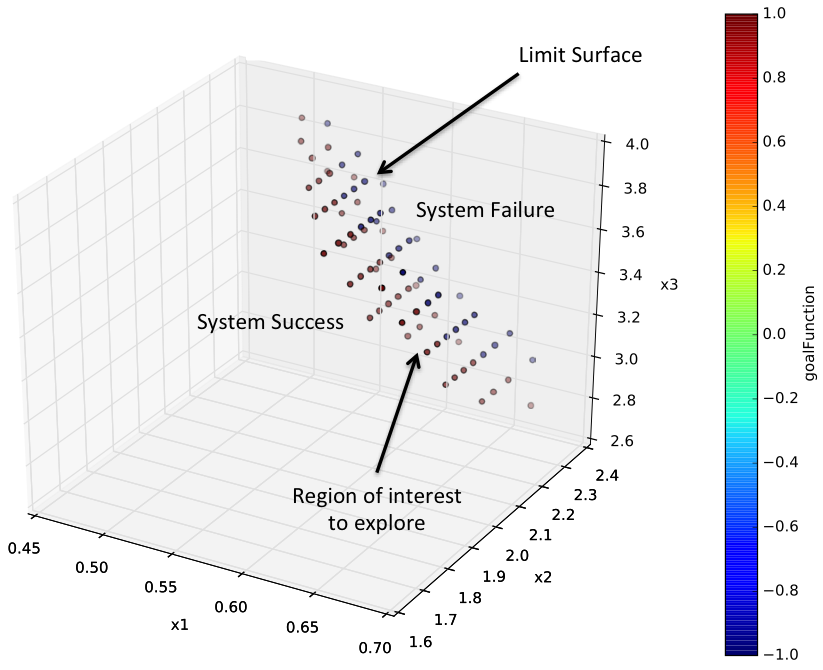
\includegraphics[width=1.0\textwidth]{pics/ExampleLSschematic.png}
  \caption{Example of limit surface in the uncertain space.}
  \label{fig:ExampleLSschematic}
\end{figure}

In the case of the ``Limit
Surface (LS) Search method'', a ROM is used to
determine the location in the input space where further observations are most
informative to establish the location of the LS, then code runs are
executed on those locations and the ROM updated. The process
continues until the location of the LS is established within a certain tolerance.

%%%%%%%%%
%%%%%%%%% Limit Surface Concept and Properties
%%%%%%%%%
\subsubsection{Limit Surface Theory}
\label{sec:LSconcept}

To properly explain the LS concept and relative properties,
it is necessary to analyze the idea behind the LSs, firstly, from a
mathematical and, secondly, from a practical point of view.
Consider a dynamic system that is represented in the phase space by the Eq.~\ref{eq:dThetaOverDT} in Section~\ref{sec:RAVENconcept}.
The equation can be rewritten as follows:
\begin{equation}
\label{eq:ThetaXPT}
\frac{\partial \overline{\theta} }{\partial t}=\overline{H}\left (  \overline{x},\overline{p},t \right )
\end{equation}
where:
\begin{itemize}
  \item $\overline{\theta}$ represents the coordinate of the system in the
  phase space
  \item $\left (  \overline{x},\overline{p},t \right )$ independent variables
  that are separated, respectively, in spatial, temporal, and parametric
  space (distinction between $\left (  \overline{x},\overline{p},t \right )$ is purely based on engineering considerations).
\end{itemize}
Now it is possible to introduce the concept of ``goal'' function, $C$. $C$
is a binary function that, based on the response of the system, can
assume the value $0$ (false) to indicate that the system is properly
available (e.g., system success) and $1$ (true) to indicate that the
system is not available (e.g., failure of the system):
\begin{equation}
C\left (\overline{\theta}, \overline{x},\overline{p},t \right ) = C\left (H\left(\overline{x},\overline{p},t \right), \overline{x},\overline{p},t \right ) = C\left ( \overline{x},\overline{p},t \right )
\end{equation}
Without loss of generality, lets assume
that $C$ does not depend on time (e.g. $C\leftarrow
\int_{t_{0}}^{t_{end}}dtC\left(  \overline{x},\overline{p},t \right )$):
\begin{equation}
  \label{eq:goalFunction}
  C = C\left (\overline{x},\overline{p}\right )
\end{equation}
To simplify the mathematical description of the LS concept, it is
possible to hypothesize that the
equation describing the PDF time evolution of the system in the phase
space is of type Gauss
Codazzi (in its Liouville’s derivation)~\cite{MathFrameworkMC2013}, which allows ensuring that all the
stochastic phenomena in
the system are representable as PDFs in the uncertain domain
(see Section~\ref{sec:RAVENconcept}),. This allows combining the
parametric space with the initial condition space:
\begin{equation}
  \label{eq:goalFunctionCodazzi}
  \begin{matrix}
  \left ( \overline{x} \right ) \leftarrow \left ( \overline{x},\overline{p} \right ) \\
  C\left ( \overline{x} \right ) \leftarrow C\left ( \overline{x},\overline{p} \right )
  \end{matrix}
\end{equation}

This assumption is rarely violated, for example for those systems that
present an intrinsic
stochastic behavior (e.g., the dynamic of a particle of dust in the air
where it continuously and
randomly interacts with the molecules of air that ``move'' with different velocities and in different
and random directions). In most of the cases of interest in the safety analysis, the above
mentioned assumption is correct. The full heuristic approach to the characterization of system stochastic behaviors is reported in Section~\ref{sec:RAVENconcept}.
\\Under the above simplifications, it is possible to identify the region of the input space ($V$)
leading to a specific outcome of the ``goal'' function. For example, it can be defined
the failure region $V_{F}$ as the region of the input space where $C=1$:
\begin{equation}
 \label{eq:failureRegion}
V_{F}=\left \{ \forall \overline{x} | C\left ( \overline{x} \right ) = 1 \right \}
\end{equation}
The definition of the complementary of the failure region is obviously:
\begin{equation}
V_{F}^{c}=\left \{ \forall \overline{x} | C\left ( \overline{x} \right ) = 0 \right \}
\end{equation}
Its boundary is the named LS:
\begin{equation}
L_{S}= \partial V_{F}^{c}= \partial      \left \{ \forall \overline{x} | C\left ( \overline{x} \right ) = 1 \right \}
\end{equation}

The identification of the LS location is necessary to identify boundary regions for which the system under consideration will or will not exceed certain FOMs (e.g., operative margins).
\\The LS location is extremely important for design optimization and, in addition, its informative content can be used to analyze the system to characterize its behavior from a stochastic point of view. Consider $\overline{x} \in V$ and $\overline{x}\sim \overline{X}$,
where $\overline{x}$ is the random variate realization of the stochastic variable $\overline{X}$.
If $pdf_{\overline{X}}\left ( \overline{x} \right ) $ is the probability density function of $ \overline{X}$, the failure probability of the system $\left ( P_{F} \right )$ is:
\begin{equation}
\label{eq:probabilityFailure}
P_{F} = \int_{V}d\overline{x}C\left ( \overline{x} \right )pdf_{\overline{X}}\left ( \overline{x} \right ) = \int_{V_{F}+V_{F}^{c}}d\overline{x}C\left ( \overline{x} \right )pdf_{\overline{X}}\left ( \overline{x} \right )
\end{equation}
And, based on the definition given in Equations~\ref{eq:goalFunctionCodazzi} and \ref{eq:failureRegion}:
\begin{equation}
 \label{eq:failureProbIntegral}
 \int_{V_{F}}d\overline{x}pdf_{\overline{X}}\left ( \overline{x} \right )
 \end{equation}
Equations \ref{eq:probabilityFailure} and \ref{eq:failureProbIntegral} are summarized by stating that the system failure probability is
equivalent to the probability of the system being in the uncertain
subdomain (region of the input space) that leads to a failure pattern.
This probability is equal to the probability-weighted hyper-volume that is surrounded by the LS (see Figure ~\ref{fig:ProbabilityFailureLSExample}).
\begin{figure}[h!]
  \centering
  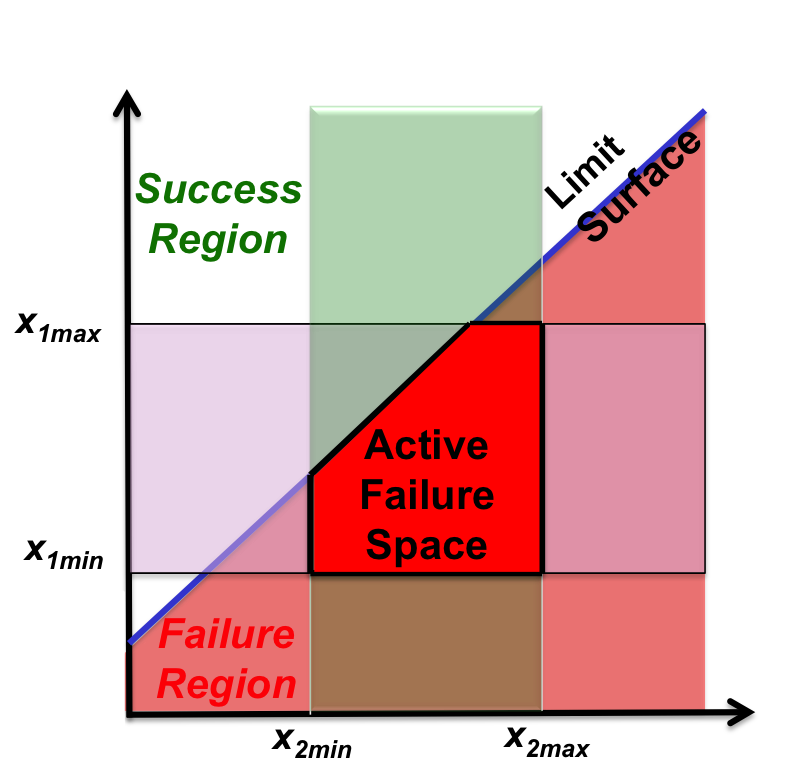
\includegraphics[width=1.0\textwidth]  {pics/ProbabilityFailureLSExample.png}
  \caption{Example of limit surface probability of failure region.}
  \label{fig:ProbabilityFailureLSExample}
\end{figure}
\\It is beneficial for better understanding to assess the LS concept through an example related to the safety of an Nuclear Power Plant (NPP).
As an example, consider a station black out (SBO) scenario in an NPP. Suppose that the only uncertain parameters are:
\begin{itemize}
  \item $t_{F}$: Temperature that would determine the failure of the fuel cladding
  \item $rt_{DGs}$: Recovery time of the diesel generators (DGs) that
  can guarantee, through the emergency core cooling system (ECCS),
  the removal of the decay heat.
\end{itemize}
And, the corresponding CDF (uniform) is:

\begin{equation}
t_{F}\sim pdf_{T_{F}}\left ( T_{F} \right )=\left\{\begin{matrix}
0 & if \: t_{F}< t_{F_{min}} \\
\frac{1}{\left ( t_{F_{max}}- t_{F_{min}} \right )=\Delta t_{F}} & \\
0 & if \: t_{F}>  t_{F_{max}}
\end{matrix}\right.
\end{equation}
%
%
\begin{equation}
rt_{DGs}\sim pdf_{RT_{DGs}}\left ( rt_{DGs} \right )=\left\{\begin{matrix}
0 & if \: rt_{DGs}<rt_{DGs_{min}}   \\
\frac{1}{\left ( rt_{DGs_{max}} - rt_{DGs_{min}} \right )=\Delta rt_{DGs}} & \\
0 & if \: rt_{DGs}>rt_{DGs_{max}}
\end{matrix}\right.
\end{equation}
For simplicity, assume that the clad temperature is a quadratic function of the DG recovery time in an SBO scenario:
\begin{equation}
  t = t_{0}+\alpha \times rt_{DGs}^{2}
\end{equation}
and that the  $ t_{F_{min}} > t_{0}+\alpha \times rt_{DGs_{min}}^{2}$
and $t_{F_{max}} < t_{0}+\alpha \times rt_{DGs_{max}}^{2}$.
The LS, failure region, and active part of the failure region (failure region with non-zero probability) are illustrated, for example, in Figure~\ref{fig:ProbabilityFailureLSExample} (in agreement with the above assumptions).
\begin{figure}[h!]
  \centering
  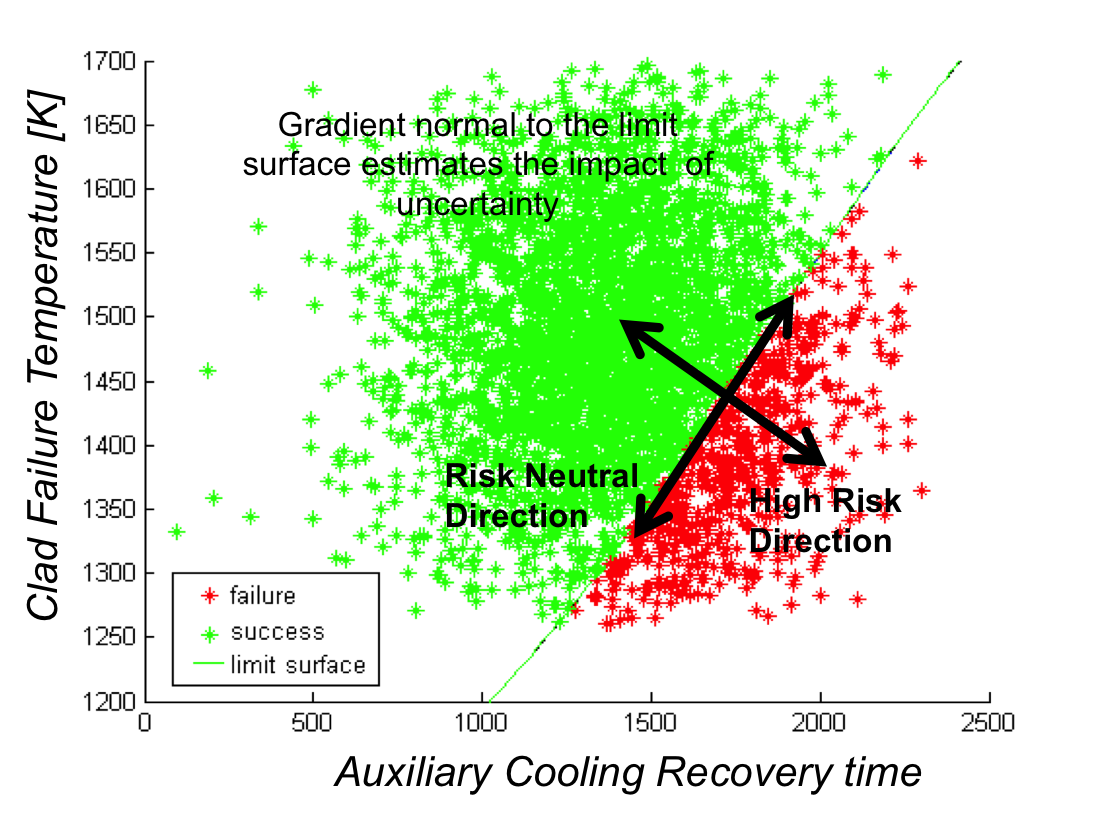
\includegraphics[width=1.0\textwidth]  {pics/ExampleLSwitRiskDirections.png}
  \caption{Example of limit surface highlighting the risk directions.}
  \label{fig:ExampleLSwitRiskDirections}
\end{figure}
In this case, the transition/failure probability is evaluated as follows:
\begin{equation}
\begin{matrix}
P_{F} = \int_{V_{F}}d\overline{x}\: pdf_{\overline{X}}\left ( \overline{x} \right )
= \int_{0}^{+\infty }d\overline{t_{F}}\: pdf_{T_{F}}\left ( T_{F} \right )\: \: \int_{\sqrt{\frac{t_{F}-t_{0}}{\alpha}}}^{+\infty } d\, rt_{DGs} \: pdf_{RT_{DGs}}\left ( rt_{DGs} \right )  =
\\
= \int_{t_{F_{min}}}^{t_{F_{max}}} dt_{F}\frac{1}{t_{F_{max}}-t_{F_{min}}}\: \: \int_{\sqrt{\frac{t_{F}-t_{0}}{\alpha}}}^{ rt_{DGs_{max}}}\: d\, rt_{DGs} \frac{1}{rt_{DGs_{max}}-rt_{DGs_{min}}} =
\\
= \frac{rt_{DGs_{max}}}{\Delta rt_{DGs}} + \frac{2\alpha}{3\left ( \Delta rt_{DGs}\Delta t_{F} \right )}
\left ( \sqrt[3/2]{\frac{t_{F_{min}}-t_{0}}{\alpha}} - \sqrt[3/2]{\frac{t_{F_{max}}-t_{0}}{\alpha}} \right )
\end{matrix}
\end{equation}

This simple example is useful to understand how the LS is defined in a practical application (that is analyzed numerically in the results Section) and how the hyper volume needs weighted with respect to the probability in the uncertain domain. An example of the computed LS is shown in Figure ~\ref{fig:ExampleLSwitRiskDirections}.
In this figure the neutral and high risk directions are highlighted.

%%%%%%%%%
%%%%%%%%% Limit Surface Search Algorithm
%%%%%%%%%
\paragraph{Limit Surface Search Algorithm}
\label{par:LSSalgorithm}
The identification of the LS location is extremely challenging,
depending on the particular physics/phenomena that are investigated.
To identify the real location of the LS, the evaluation of system
responses is needed, through the high-fidelity code (RELAP 7,
RELAP5-3D, etc.), in the full domain of uncertainty (infinite number of
combinations of uncertainties represented by the respective PDFs).
Obviously, this is not a feasible approach, and a reasonable
approximation is to locate the LS on a Cartesian N-D grid, in the
uncertain domain.

In reality, the location of the LS is not exactly determined but rather
bounded. The algorithm determines the set of grid nodes between
which the transition $0/1$ of the ``goal'' function happens. This set is
also classified with respect to the value of the ``goal'' function. With
reference to Figure~\ref{fig:LSgoalFunctionExample}, for example,
green is used for grid nodes with a
``goal'' function that equals $0$ and red when the ``goal'' function
equals $1$.
\begin{figure}[h!]
  \centering
  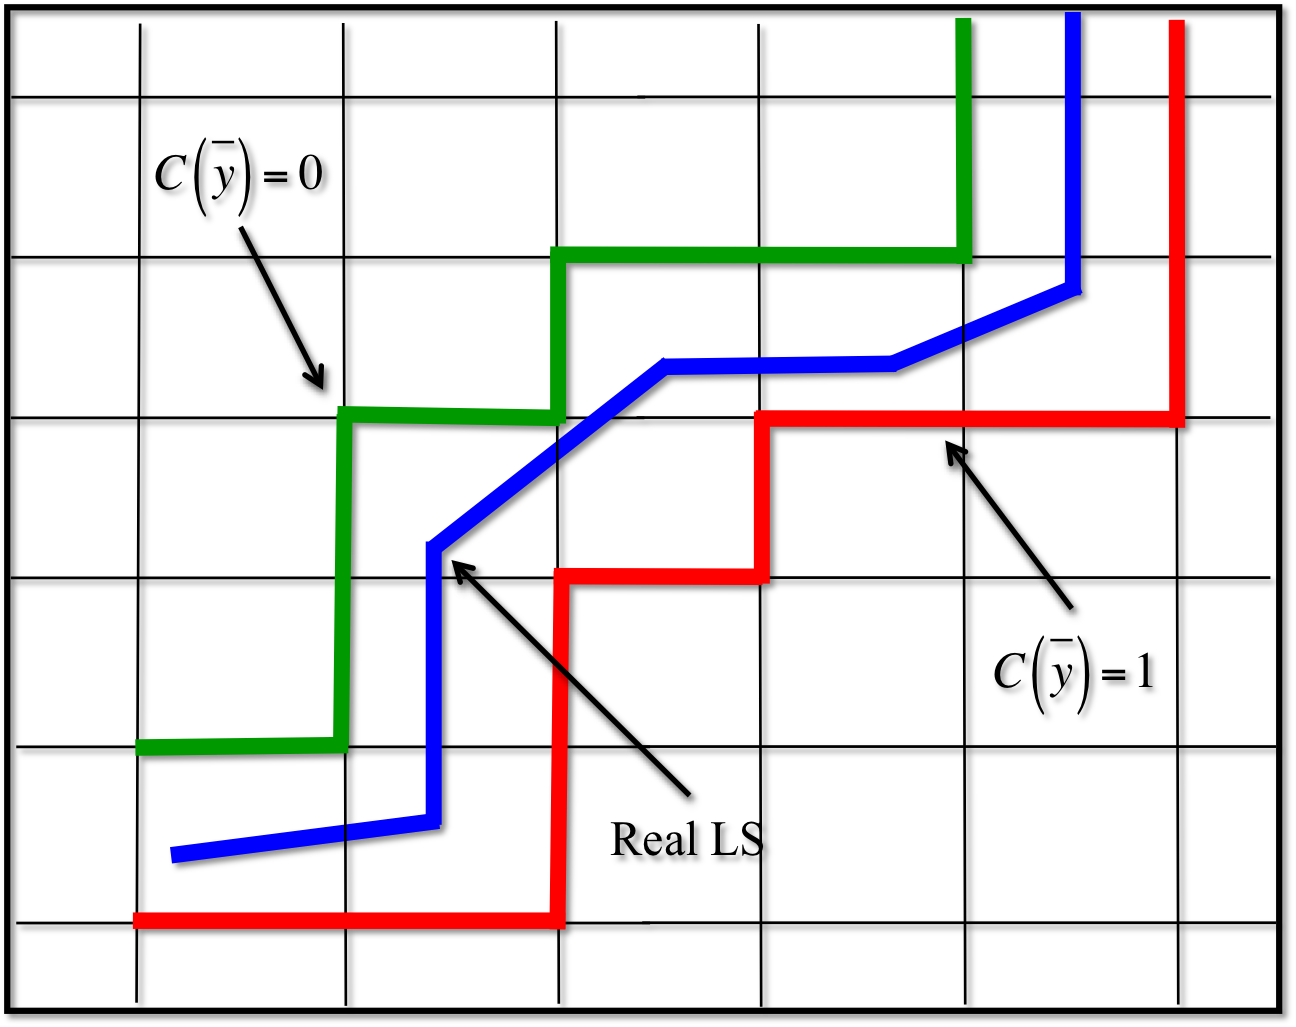
\includegraphics[width=1.0\textwidth]  {pics/LSgoalFunctionExample.png}
  \caption{Example of limit surface search evaluation grid (where $\overline{y}=\overline{\theta}$).}
  \label{fig:LSgoalFunctionExample}
\end{figure}
Each evaluation of the ``goal'' function in one of the grid nodes implies
the evaluation of the high-fidelity code (e.g. system simulator) for the
corresponding set of entries in the uncertain space. As already
mentioned, the evaluation of the high fidelity code is computationally
expensive and, in order to identify the LS, one should appraise
each point in the N-D grid covering the uncertainty space.
Discretization depends on the accuracy requested by the user. In
most cases, this approach is not feasible and, consequentially, the
process needs to be accelerated using ``predicting'' methods that are
represented by the employment of supervised learning algorithms
(i.e., ROMs).

This approach is commonly referred to as an active learning process
that ultimately results in training of a ROM of type classifier capable of
predicting the outcome of the ``goal'' function for any given point of
the uncertain space.
In an active learning process, a supervised learning algorithm is
combined with criteria to choose the next node in the N D grid that
needs explored, using the high fidelity physical model. This process is
repeated until, under a particular metric, the prediction capabilities of
the supervised learning algorithm do not improve by further increasing
the training set.

In more detail, the iterative scheme could be summarized through the following steps:
\begin{enumerate}
  \item A limited number of points in the uncertain space $\left \{
  \overline{x}_{k} \right \}$ are selected via one of the forward
  sampling strategies (e.g., stratified or Monte Carlo)
  \item The high fidelity code is used to compute the status of the
  system for the set of points in the input set:
  $
  \left \{ \overline{\theta}(t)\right \}_{k} = H\left ( \left \{ \overline{x} \right
  \}_{k},t \right )
  $.
  \item The ``goal'' function is evaluated at the phase space coordinate
  of the system:
  $\left \{ c \right \}_{k} = C\left ( \left \{ \overline{\theta}(t)\right \}_{k}
  \right )$
   \item The set of pairs $\left \{ \left ( \overline{x},c \right )_{k} \right \}$
   are used to train a ROM of type classifier, $G\left ( \left \{
   \overline{x}_{k} \right \} \right )$
   \item The ROM classifier is used to predict the values of the ``goal''
   function for all the $N$ nodes of the N-D grid in the domain space:
   \begin{equation}
   \left (G\left ( \left \{ \overline{x} \right \}_{j} \right ) \sim \left \{ c \right
   \}_{j}, j=1,...,N  \right )
    \end{equation}
    \item The values of the ``goal''  function are used to determine the
    LS location based on the change of values of  $\left \{ c \right
    \}_{j}$:
    \begin{equation}
    \left \{ c \right \}_{j}\rightarrow \partial V_{F}
     \end{equation}
     \item A new point is chosen to increase the training set and a new
     pair is generated
     \item The procedure is repeated starting from Step 3 until
     convergence is achieved. The convergence is achieved when
     there are no changes in the location of the LS after a certain
     number of consecutive iterations.
\end{enumerate}
The iteration scheme is graphically shown in
Figure~\ref{fig:LimitSurfaceAlgoFlow}.
\begin{figure}[h!]
  \centering
  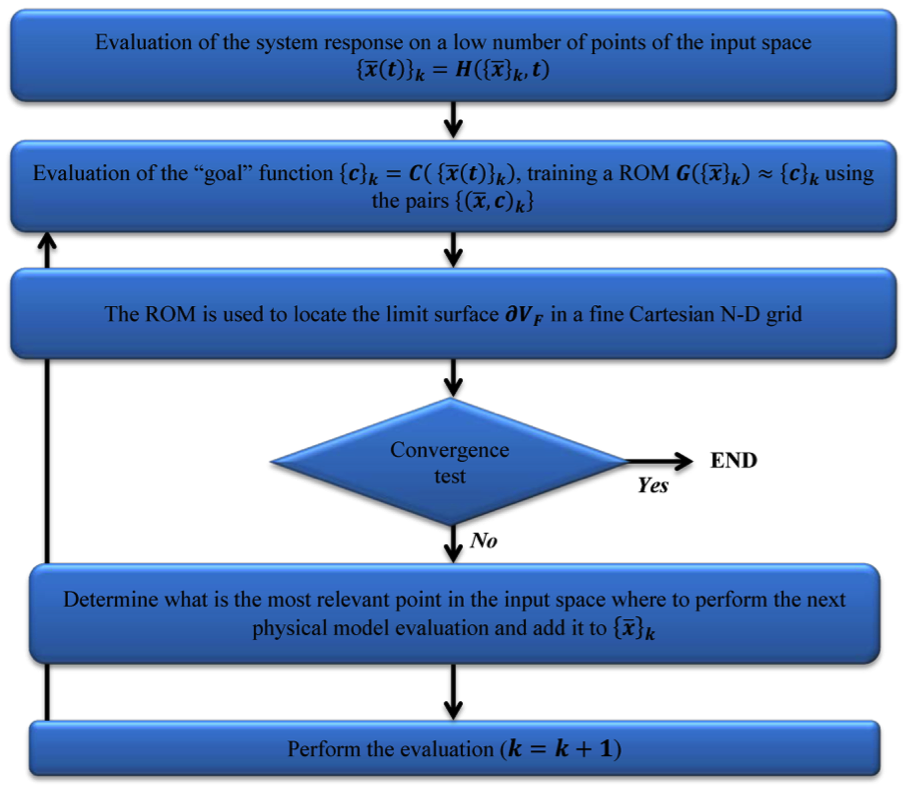
\includegraphics[width=1.0\textwidth]  {pics/LimitSurfaceAlgoFlow.png}
  \caption{Limit surface search algorithm conceptual scheme.}
  \label{fig:LimitSurfaceAlgoFlow}
\end{figure}
Note that there is an additional requirement
regarding the LS search algorithm:the LS location
has to stay constant for a certain number (user defined) of consecutive
iterations. The reason for this choice is determined by the attempt to
mitigate the effect of the build of non-linear bias in the searching
pattern. Indeed, the searching algorithm might focus too much on a
certain region of the LS while putting too few points in other zones
and completely hiding undiscovered topological features of the LS.
Regarding the strategy to choose the nodes on the N-D grid that
needs evaluated in the iterative process for the LS identification, it has
been decided to employ a metric based on the
distance between the predicted LS and the evaluations already
performed. The points on the LS are ranked based on the distance
from the closest training point already explored (the larger is the
distance the higher is the score for the candidate point), and based on
its persistence (the larger is the number of time the prediction of the
``goal'' function for that point have changed the higher is the score).
Since this approach creates a queue of ranked candidates, it could be
used also in the parallel implementation of the algorithm. When
several training points are run in parallel, it is possible that the
evaluation of one additional point does not alter dramatically the
location of the LS. Consequently, it is possible that the candidate with
the highest score is already being submitted for evaluation and
possibly the simulation is not yet completed. In this case, to avoid
submitting the same evaluation point twice, the algorithm searches
among all the ranked candidates (in descending order) for the one
that was not submitted for evaluation. Even if it is extremely unlikely
that all the candidates were submitted, in this remote event, the
method will choose the next point employing a Monte Carlo strategy.
%%%%%%%%%
%%%%%%%%% Acceleration through Multi-grid Approach
%%%%%%%%%
\paragraph{Acceleration through Multi-grid Approach}
\label{par:LSaccelerationMultiGrid}
The location of the LS, being a numerical iterative process, can be
known given a certain tolerance. As already mentioned, the LS search
is done by constructing an evaluation grid on which the acceleration
ROM is inquired. The tolerance of the iterative process determines how
the evaluation grid is discretized. Before addressing the acceleration
scheme, it is important
to introduce some concepts on the employed numerical process.
\begin{figure}[h!]
  \centering
  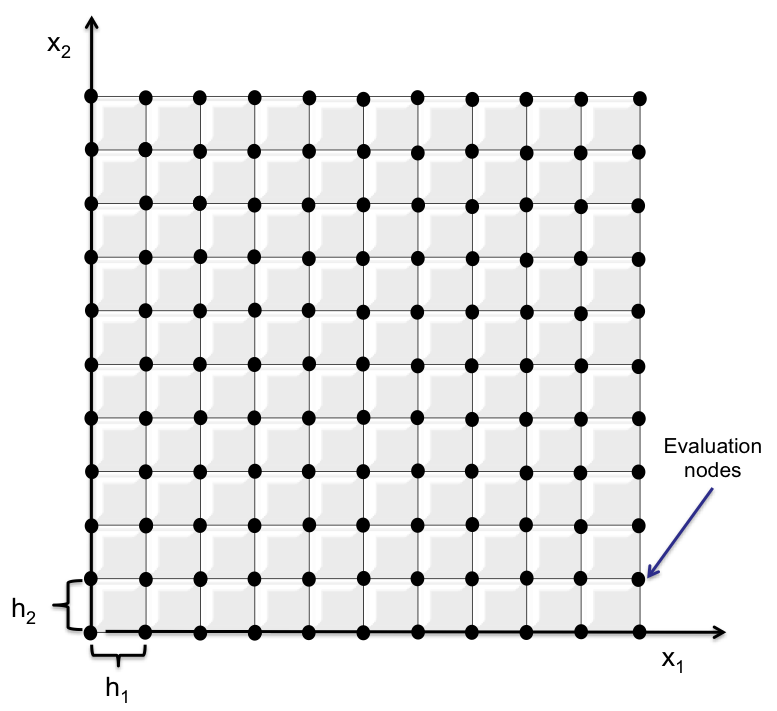
\includegraphics[width=1.0\textwidth]  {pics/DiscretizationGrid.png}
  \caption{Discretization grid.}
  \label{fig:DiscretizationGrid}
\end{figure}
\\Assume that each of $D$ dimensions of the uncertain domain is
discretized with the same number of equally-spaced nodes $N$ (see
Figure~\ref{fig:DiscretizationGrid}), with discretization size indicated
by $h_{i}$. Hence, the Cartesian grid contains $N^{D}$ individual
nodes, indexed through the multi-index vector $\overline{j} = \left (
j_{i=1\rightarrow D} \right ), j_{i} \leq N \forall i$. Introducing the
vectors  $\overline{I} = (1, ..., 1)$ and
$\overline{N} = (N, ..., N)$, the ``goal'' function is expressed on this N-
D grid as:
\begin{equation}
C\left ( \overline{x} \right ) =
\mathlarger{\sum}_{\overline{j}=\overline{I}}^{\overline{N}} \varphi_{\overline{j}}\left
( \overline{x} \right ) C\left ( \overline{x}_{\overline{j}} \right )
\end{equation}
where $\varphi_{\overline{j}}$ is the characteristic function of the hyper-volume $\Omega_{\overline{j}}$ surrounding the node
 $\overline{x}_{\overline{j}}$:
 \begin{equation}
 \varphi_{\overline{j}}\left ( \overline{x} \right ) =
\left\{\begin{matrix}
1 & if \: \overline{x} \in \Omega_{\overline{j}} \\
0 & if \: \overline{x} \notin \Omega_{\overline{j}}
\end{matrix}\right.
\end{equation}
where:
 \begin{equation}
 \label{eq:OmegaEq}
 \Omega_{\overline{j}} = \prod_{i=1}^{D}\left [ x_{j_{i}} - \frac{h_{i}}{2},
 x_{j_{i}} + \frac{h_{i}}{2}  \right ]
 \end{equation}
 The probability of the uncertain parameters is expressed as:
 \begin{equation}
 pdf_{\overline{X}}\left ( \overline{x} \right ) =
\mathlarger{\sum}_{\overline{j}=\overline{I}}^{\overline{N}}
\varphi_{\overline{j}}\left ( \overline{x} \right )
pdf_{\overline{X}}\left ( \overline{x}_{\overline{j}} \right )
 \end{equation}
Following the approach briefly explained in Section
\ref{sec:LSconcept}, the probability of the event (e.g., failure) could be
expressed as:
 \begin{equation}
 \label{eq:Pf}
  P_{F}=\left ( \prod_{i=1}^{D}h_{i} \right )
  \mathlarger{\sum}_{\overline{j}=
  \overline{I}}^{\overline{N}}pdf_{\overline{X}}\left (
  \overline{x_{\overline{j}}} \right )
  C\left ( \overline{x}_{\overline{j}} \right )
 \end{equation}
Under certain assumptions, the concept of active hyper-volume
$V_{A}$ as the region of the input space identified by the support of
the uncertain parameters’ probability density functions
$pdf_{\overline{X}}\left ( \overline{x} \right )$ could be introduced;
Equation ~\ref{eq:Pf} is recast, using a Taylor expansion, as follows:
 \begin{equation}
P_{F}= \int_{V} C\left ( \overline{x} \right )\: pdf_{\overline{X}}\left (
\overline{x}  \right )\: d\overline{x} =\int_{V_{A}}C\left ( \overline{x}
\right )\:
\left [
\mathlarger{\sum}_{\overline{j}=\overline{I}}^{\overline{N}}\varphi_{\overline{j}}\left (
\overline{x} \right )
\left ( pdf_{\overline{X}}\left ( \overline{x}_{\overline{j}} \right ) +
\mathlarger{\sum}_{i=1}^{D} \frac{\partial pdf_{\overline{X}}}{\partial x_{i}}|
_{\overline{x}_{\overline{j}}} \: \left ( x_{i} - x_{j_{i}} \right ) \right ) \right
] d\overline{x}
 \end{equation}
And, considering the evaluation grid as:
\begin{equation}
\label{eq:PfEq}
P_{F}= \mathlarger{\sum}_{\begin{matrix}
\overline{j}=\overline{I} \\ \overline{x}_{\overline{j}} \in V_{A} \end{matrix}}^{\overline{N}}
\int_{\overline{x}_{\overline{j}} - \overline{h}/2}^{\overline{x}_{\overline{j}} + \overline{h}/2} C\left ( \overline{x} \right )\:
\left [  \mathlarger{\sum}_{\overline{j}=\overline{I}}^{\overline{N}}\varphi_{\overline{j}}\left ( \overline{x} \right )
\left ( pdf_{\overline{X}}\left ( \overline{x}_{\overline{j}} \right ) +
\mathlarger{\sum}_{i=1}^{D} \frac{\partial pdf_{\overline{X}}}{\partial x_{i}}|_{\overline{x}_{\overline{j}}} \: \left ( x_{i} - x_{j_{i}} \right ) \right ) \right ] d\overline{x}
\end{equation}
At this point, it is possible to label, in the active hyper-volume, the sub-
domain identified by the nodes where the ``goal'' function
$C(\overline{x})$ changes its value (the frontier nodes between the
region where $C(\overline{x})=1$ and $C(\overline{x})=0$) $V_{A} \cap
V_{\partial V_{F}}$.
\\ Consequentially, it is possible to identify the sub-domains in which the  ``goal''  function $C(\overline{x})$ is equal to $0$ ($V_{A} \cap V_{\partial V_{C(\overline{x})=0}} \notin V_{A} \cap V_{\partial V_{F}}$):

\begin{equation}
\mathlarger{\sum}_{\begin{matrix}
\overline{j}=\overline{I} \\ \overline{x}_{\overline{j}} \in V_{A} \cap V_{C(\overline{x})=0} \end{matrix}}^{\overline{N}}
\int_{\overline{x}_{\overline{j}} - \overline{h}/2}^{\overline{x}_{\overline{j}} + \overline{h}/2} C\left ( \overline{x} \right )\:
\left ( pdf_{\overline{X}}\left ( \overline{x}_{\overline{j}} \right ) +
\mathlarger{\sum}_{i=1}^{D} \frac{\partial pdf_{\overline{X}}}{\partial x_{i}}|_{\overline{x}_{\overline{j}}} \: \left ( x_{i} - x_{j_{i}} \right ) \right )   d\overline{x}
\end{equation}
in which the  ``goal''  function $C(\overline{x})$ is equal to $1$ ($V_{A} \cap V_{\partial V_{C(\overline{x})=1}} \notin V_{A} \cap V_{\partial V_{F}}$):
\begin{equation}
\begin{matrix}
\mathlarger{\sum}_{\begin{matrix}
\overline{j}=\overline{I} \\ \overline{x}_{\overline{j}} \in V_{A} \cap V_{C(\overline{x})=1} \end{matrix}}^{\overline{N}}
\int_{\overline{x}_{\overline{j}} - \overline{h}/2}^{\overline{x}_{\overline{j}} + \overline{h}/2} C\left ( \overline{x} \right )\:
\left ( pdf_{\overline{X}}\left ( \overline{x}_{\overline{j}} \right ) +
\mathlarger{\sum}_{i=1}^{D} \frac{\partial pdf_{\overline{X}}}{\partial x_{i}}|_{\overline{x}_{\overline{j}}} \: \left ( x_{i} - x_{j_{i}} \right ) \right )   d\overline{x} =
\\
= \mathlarger{\sum}_{\begin{matrix}
\overline{j}=\overline{I} \\ \overline{x}_{\overline{j}} \in V_{A} \cap V_{C(\overline{x})=1} \end{matrix}}^{\overline{N}}
\int_{\overline{x}_{\overline{j}} - \overline{h}/2}^{\overline{x}_{\overline{j}} + \overline{h}/2}
\left ( pdf_{\overline{X}}\left ( \overline{x}_{\overline{j}} \right ) +
\mathlarger{\sum}_{i=1}^{D} \frac{\partial pdf_{\overline{X}}}{\partial x_{i}}|_{\overline{x}_{\overline{j}}} \: \left ( x_{i} - x_{j_{i}} \right ) \right )   d\overline{x}
\end{matrix}
\end{equation}
Equation ~\ref{eq:PfEq} is now expressed as:
 \begin{equation}
 \label{eq:PfEqFinal}
 \begin{matrix}
P_{F} = \mathlarger{\sum}_{\begin{matrix}
\overline{j}=\overline{I} \\ \overline{x}_{\overline{j}} \in V_{A} \cap
V_{C(\overline{x})=1} \end{matrix}}^{\overline{N}}
\left ( \prod_{i=1}^{D}
 h_{i} \right )
\: pdf_{\overline{X}} ( \overline{x}_{\overline{j}}) + O(h^{N+1}) +
 \\
 + \mathlarger{\sum}_{\begin{matrix}
\overline{j}=\overline{I} \\ \overline{x}_{\overline{j}} \in V_{A} \cap
V_{\partial V_{f}} \end{matrix}}^{\overline{N}}
\int_{\overline{x}_{\overline{j}} -
\overline{h}/2}^{\overline{x}_{\overline{j}} + \overline{h}/2} C\left (
\overline{x} \right )\: \left ( pdf_{\overline{X}}\left (
\overline{x}_{\overline{j}} \right ) +
\mathlarger{\sum}_{i=1}^{D} \frac{\partial pdf_{\overline{X}}}{\partial
x_{i}}|_{\overline{x}_{\overline{j}}} \: \left ( x_{i} - x_{j_{i}} \right ) \right )
d\overline{x}
\end{matrix}
 \end{equation}
As inferred from Equation ~\ref{eq:PfEqFinal}, the process is bounded if the
surface area-to-volume ratio (amount of surface area per unit volume) is
in favor of the volume:
\begin{equation}
\label{eq:convergenceCondition}
\mathlarger{\sum}_{\begin{matrix}
\overline{j}=\overline{I} \\ \overline{x}_{\overline{j}} \in V_{A} \cap
V_{C(\overline{x})=1} \end{matrix}}^{\overline{N}}
\left ( \prod_{i=1}^{D}
 h_{i} \right )
\: pdf_{\overline{X}} ( \overline{x}_{\overline{j}})
\gg
\sum_{\begin{matrix}
\overline{j}=\overline{I} \\ \overline{x}_{\overline{j}} \in V_{A} \cap
V_{\partial V_{f}} \end{matrix}}^{\overline{N}}
\left | \int_{\overline{x}_{\overline{j}} -
\overline{h}/2}^{\overline{x}_{\overline{j}} + \overline{h}/2}   pdf_{\overline{X}}\left (
\overline{x}_{\overline{j}} \right )  \right |
d\overline{x}
\end{equation}
If the grid is built in the transformed space of probability (i.e., replacing the measure $d\overline{x}$ with $d \overline{\mu }\: \: pdf_{\overline{X}}\left ( \overline{x}_{\overline{j}} \right )$ the condition expressed in Equation ~\ref{eq:convergenceCondition} is reduced:
\begin{equation}
number \: \:  nodes \in V_{A} \cap V_{C(\overline{x})=1} \gg number \: \:  nodes  \in V_{A} \cap V_{\partial V_{F}}
\end{equation}
This means that error is bounded by the total probability contained in the cells on the frontier of the LS.

Based on this derivation, it is clear how important it is to keep the
content of the total probability on the frontier of the LS as low as
possible, and simultaneously, increase the importance of the volume of
the failure/event region as much as possible (to improve the surface
area-to-volume ratio).

To do that, the step size in probability should be significantly
reduced ( $h_{i}^{p} \rightarrow 0^{+}$). Even if this is theoretically
feasible, it is computational inapplicable. To approach a similar result, it
is possible to learn from other numerical methods that use the
technique of adaptive meshing for the resolution of the partial
differential equation system (e.g., finite element methods).

For this reason, an acceleration scheme was designed and developed
employing a multi-grid approach. The main idea, it is to recast the
iterative process in two different sub-sequential steps. Firstly,
performing the LS search on a coarse evaluation grid, and once
converged, adaptively refining the cells that lie on the frontier of the LS
($V_{A} \cap V_{\partial V_{F}}$) and, consequentially, converging on
the new refined grid.
\\The iteration scheme is graphically shown in
Figure~\ref{fig:LimitSurfaceMultiGridAlgoFlow}.
\begin{figure}[h!]
  \centering
  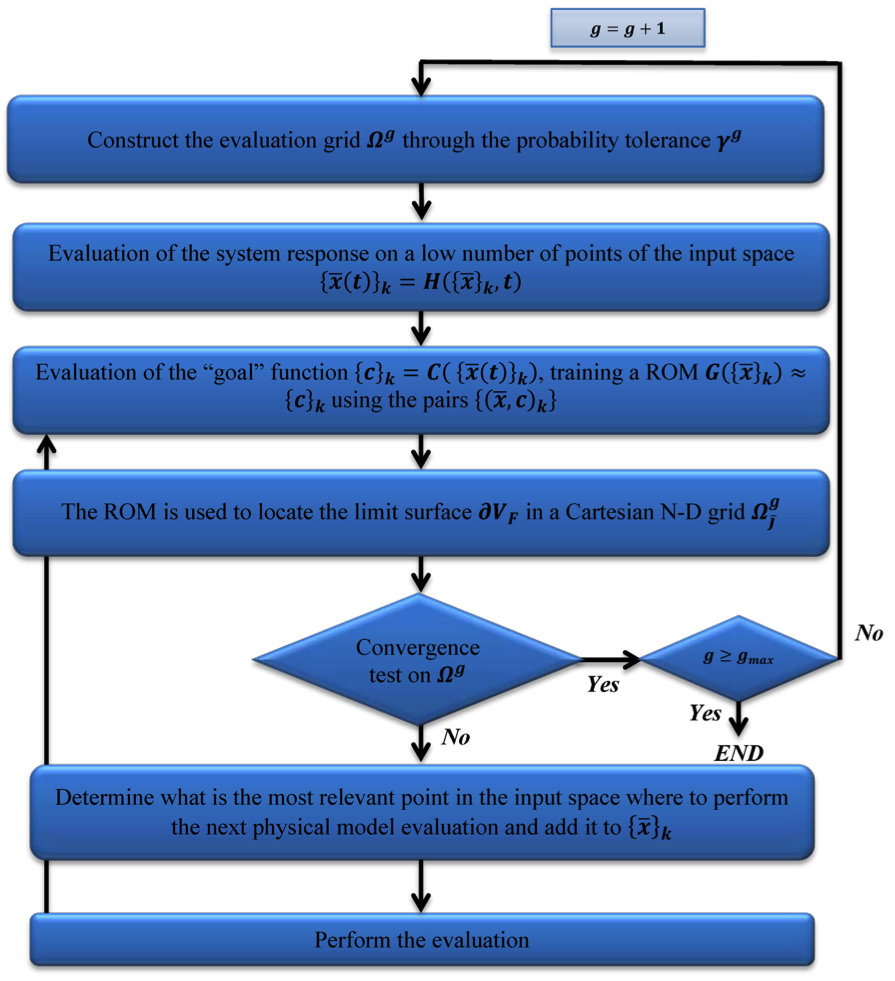
\includegraphics[width=1.0\textwidth]  {pics/LimitSurfaceMultiGridAlgoFlow.png}
  \caption{Multi-grid limit surface search scheme.}
  \label{fig:LimitSurfaceMultiGridAlgoFlow}
\end{figure}
In more detail, the iterative scheme could be summarized through the
following steps:
\begin{enumerate}
  \item The user specifies two tolerances in probability $(CDF):
  \gamma^{g=1}$ for the initial coarse grid and $\gamma^{g=2}$
  for the refined grid, where  $ \gamma^{g=1} >  \gamma^{g=2}$;
  \item Following Equation ~\ref{eq:OmegaEq}, the initial coarse evaluation
  grid $\Omega^{1}$ is constructed ($N^{g=1}$ total nodes). The
  discretization of this grid is done to have cells with a content of
  probability equal to $\gamma^{g=1}$.
  \item A limited number of points in the uncertain space $\left \{
  \overline{x}_{k} \right \}$ are selected via one of the forward
  sampling strategies (e.g., stratified or Monte Carlo).
  \item The high fidelity code is used to compute the status of the
  system for the set of points in the input set:
  $
  \left \{ \overline{\theta}(t)\right \}_{k} = H\left ( \left \{ \overline{x} \right
  \}_{k},t \right )
  $.
  \item The ``goal'' function is evaluated at the phase space coordinate
  of the system:
  $\left \{ c \right \}_{k} = C\left ( \left \{ \overline{\theta}(t)\right \}_{k}
  \right )$.
   \item The set of pairs $\left \{ \left ( \overline{x},c \right )_{k} \right \}$
   are used to train a ROM of type classifier, $G\left ( \left \{
   \overline{x}_{k} \right \} \right )$.
   \item The ROM classifier is used to predict the values of the ``goal''
   function for all the $N^{g=1}$ nodes of the N-D grid in the domain
   space:
   \begin{equation}
   \left (G\left ( \left \{ \overline{x} \right \}_{j} \right ) \sim \left \{ c \right
   \}_{j}, j=1,...,N^{g=1}  \right )
    \end{equation}
    \item The values of the ``goal''  function are used to determine the
    LS location based on the change of values of  $\left \{ c \right
    \}_{j}$:
    \begin{equation}
    \left \{ c \right \}_{j}\rightarrow \partial V_{F}
     \end{equation}
     \item A new point is chosen to increase the training set and a new
     pair is generated.
     \item The procedure is repeated starting from Step 5 until
     convergence is achieved on grid $\Omega^{g}$.The convergence
     is reached when there are no changes in the location of the LS
     after a certain number of consecutive iterations (user defined).
     \item When the convergence is achieved on the coarse grid
     $\Omega^{g=1}$, all the cells that lie on the frontier of the LS
     ($V_{A} \cap V_{\partial V_{F}}$) are refined to contain an amount of
     probability equal to  $\gamma^{g=2}$.
     \item Steps 7 through 9 are performed based on the new refined
     grid. Finally, the process starts again by performing Steps 5
     through 10, until the convergence is achieved in the refined grid.
\end{enumerate}
As shown in Figure~\ref{fig:LimitSurfaceMultiGridAlgoFlow}, the
algorithm consists in searching the location of the LS proceeding with
subsequential refinement of the sub-domain, in the active space, that
contains the LS. In this way, the computational burden is kept as low as
possible. In addition, another advantage of this approach is that, since
the refinement grid represents a constrained domain, the sub-
sequential ROM training process can be regularized, since the LS
between an iteration and the other can move, at maximum, within the
refinement domain.


\section{Reduced Order Modeling}
\label{sec:ROMs}
To provide a very simple idea of a ROM, assume that the final
response space of a physical system is governed by the transfer
function $H \left (  \overline{x}\right)$ (see Section
~\ref{sec:mathBackground}), which, from a practical point of
view, represents the outcome of the system based on the initial
conditions  $\overline{x}$. Now, sample the domain of variability of the
initial conditions $\overline{x}$ to create a
set of $N$ realizations of the input and response space $ \left ( \left (
\overline{x}_{i}, H \left (  \overline{x}_{i}\right) \right), i=1,N \right)$,
named ``training'' set. Based on the data set generated, it is possible
to construct a mathematical representation $G\left ( \overline{x}:
\overline{x}_{i}\right)$ of the
real system $H \left (  \overline{x}\right)$, which will approximate its
response (see Figure~\ref{fig:ROMexampleOfPhysicalSystem}):
\begin{equation}
\label{eq:regressor}
G\left ( \overline{x} \right ):\overline{x}_{i} \rightarrow G\left ( \overline{x}_{i} \right ) \cong H\left ( \overline{x}_{i} \right )
\end{equation}
The ROMs reported above are generally named ``regressors'', among
which all the most common data fitting algorithms are found (e.g.,
least square for construction of linear models).
An important class of ROMs for the work presented here after is the
one containing the so called ``classifiers''. A classifier is a ROM that is
capable of representing the system behavior from a binary point of
view (e.g., event happened/not happened or failure/success). It is a
model (set of equations) that identifies to which category an object
belongs in the feature (input) space. Referring to the example that
brought to Equation ~\ref{eq:regressor}, a classifier can be formally represented as follows (see
Figure~\ref{fig:ROMClassifierExampleOfPhysicalSystem}):
\begin{figure}[h!]
  \centering
  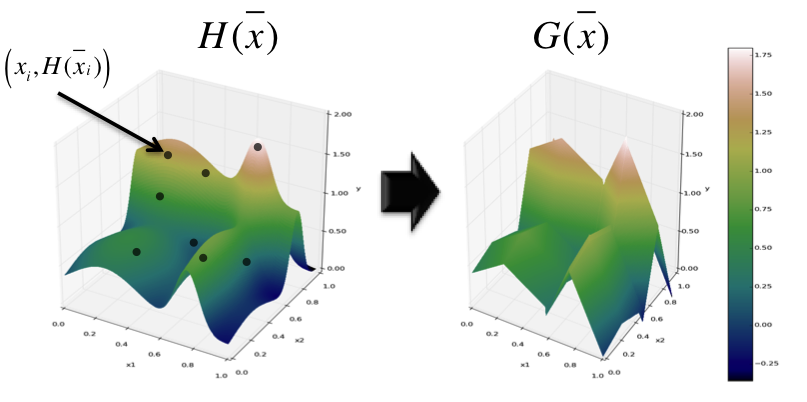
\includegraphics[width=1.0\textwidth]  {pics/ROMexampleOfPhysicalSystem.png}
  \caption{Example of reduced order model representation of physical system (regression).}
  \label{fig:ROMexampleOfPhysicalSystem}
\end{figure}
\begin{figure}[h!]
  \centering
  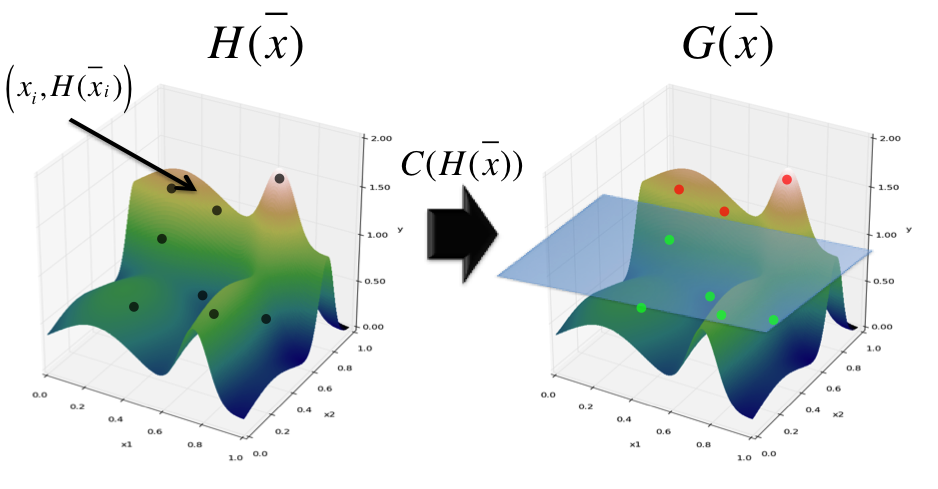
\includegraphics[width=1.0\textwidth]  {pics/ROMClassifierExampleOfPhysicalSystem.png}
  \caption{Example of reduced order model representation of physical system (classifier).}
  \label{fig:ROMClassifierExampleOfPhysicalSystem}
\end{figure}

\begin{equation}
\label{eq:classifier}
G\left ( \overline{x} \right ):\overline{x}_{i} \rightarrow G\left ( \overline{x}_{i} \right ) \cong
C \left ( H\left ( \overline{x}_{i} \right ) \right )
\end{equation}

The function $C\left (  H\left ( \overline{x}_{i}  \right ) = \overline{\theta}
\right ) $ is the so called ``goal'' function that is able to recast the
response of the system $H\left ( \overline{x}_{i}  \right )$ into a binary
form (e.g., failure/success). As an example, referring to
Figure~\ref{fig:ROMClassifierExampleOfPhysicalSystem}, the
``goal'' function would be:
\begin{equation}
\label{eq:goalFunctionClassifier}
C\left (   \overline{\theta}  \right ) = \left\{\begin{matrix}
1 & if \: \overline{\theta}>1.0 \\
0 &  if \: \overline{\theta} \leq 1.0
\end{matrix}\right.
\end{equation}
Hence, the ROM of type classifier $G\left (  \overline{x} \right )$  will operate in the space transformed through the ``goal''  function $C\left (   \overline{\theta}  \right )$.
\\The classifiers and regressors can be categorized into two main classes:
\begin{itemize}
  \item Model-based algorithms
  \item Data-based algorithms
\end{itemize}
In the first class, the created ROM aims to approximate the response
of the system as a function of the input parameters. These algorithms
construct a functional representation of the system. Examples of such ROM type are Support Vector Machines (SVMs), Kriging-based regressors, discriminant-based models, and polynomial chaos.

On the other side, data-based algorithms do not build a response-
function-based ROM but classify or predict the response of the
system from the neighborhood graph constructed from the training
data, without any dependencies on a particular prediction model.
These algorithms directly build a neighborhood structure as the
ROM (e.g., a relaxed Gabriel graph) on the initial training data. Examples of such ROM type are nearest neighbors and decision trees.

\textcolor{red}{\\It is important to NOTE that RAVEN uses a Z-score normalization of the training data before
  constructing most of the ROMs:
\begin{equation}
  \mathit{\mathbf{X}} = \frac{(\mathit{\mathbf{X}}-\mu )}{\sigma }
\end{equation}
 }
In order to identify which ROMs get trained with data normalized by the previous reported normalization approach, please refer to the RAVEN user manual \cite{RAVENuserManual}.

RAVEN has support of several different ROMs,
such as:
\begin{enumerate}
  \item \textit{Nearest Neighbors approaches}
  \item \textit{Support Vector Machines}
  \item \textit{Inverse Weight regressors}
  \item \textit{Spline regressors }, etc.
\end{enumerate}
In this section only few of them are going to be explained. 

\subsection{Gaussian Process Models}
\label{sec:GPM}
Gaussian Processes (GPs)~\cite{Rasmussen_GPM} are algorithms that extend multivariate Gaussian distributions to infinite dimensionality. A Gaussian process generates a data set located throughout some domain such that any finite subset of the range follows a multivariate Gaussian distribution. Now, the n observations in an arbitrary data set, $y={y_1,\ldots,y_n}$, can always be imagined as a single point sampled from some multivariate ($n$-variate) Gaussian distribution.
What relates one observation to another in such cases is just the covariance function, $k(x,x')$. A popular choice is the squared exponential:
\begin{equation}
k(x,x')=\sigma_{f}^{2}  exp \left [ \frac{-(x-x')^2}{2 l^2} \right ]
\end{equation}
where the maximum allowable covariance is defined as $\sigma_{f}^{2}$; this should be high for functions that cover a broad range on the y axis. If $x \simeq x'$, then $k(x,x')$ approach this maximum meaning $f(x)$ is very correlated to $f(x')$. On the other hand, if $x$ is very distant from $x'$, then $k(x,x' ) \simeq 0$ (i.e., the two points cannot see each other.
So, for example, during interpolation at new $x$ values, distant observations will have negligible effect). How much effect this separation has will depend on the length parameter $l$.
Each observation $y$ can be thought of as related to an underlying function $f(x)$ through a Gaussian noise model:
\begin{equation}
y=f(x)+N(0,\sigma_{n}^{2})
\end{equation}
The new kernel function can be written as:
\begin{equation}
k(x,x')=\sigma_{f}^{2}  exp \left [ \frac{-(x-x')^2}{2 l^2} \right ] + \sigma_{n}^{2} \delta(x,x')
\end{equation}
So given $n$ observations $y$, the objective is to predict the value $y_*$ at the new point $x_*$. This process is performed by following this sequence of steps:
\begin{enumerate}
\item Calculate three matrices:
\begin{equation}
K=\begin{bmatrix}
k(x_1,x_1) &  \ldots & k(x_1,x_n)\\
\vdots  & \ddots &\vdots  \\
k(x_n,x_1) &  \ldots & k(x_n,x_n)
\end{bmatrix}
\end{equation}
\begin{equation}
K_*= \begin{bmatrix}
k(x_*,x_1) & \ldots & k(x_*,x_n)
\end{bmatrix}
\end{equation}
\begin{equation}
K_{**}=k(x_*,x_*)
\end{equation}
\item The basic assumption of GPM is that:
\begin{equation}
\begin{bmatrix}
y\\
y_*
\end{bmatrix}
=\mathcal{N}(0,\begin{bmatrix}
K & K_{*}^{T}\\
K_* & K_{**}
\end{bmatrix})
\end{equation}
\item The estimate $\bar{y_*} $ for $y_*$ is the mean of this distribution
\begin{equation}
\bar{y_*}=K_* K^{-1}y
\end{equation}
\item The uncertainty associated to the estimate $\bar{y_*} $ can be expressed in terms of variance of  $y_*$:
\begin{equation}
var(y_*)=K_{**}-k_* K^{-1} K_{*}^{T}
\end{equation}
\end{enumerate}

\subsection{Support Vector Machines}
\label{sec:SVM}
The Support Vector Machine (SVM)~\cite{SVM_Burges} classifier is a methodology that aims to determine the optimal separation hyperplane between data sets having different labels.
The training data consist of $N$ data points $(x_i,y_i)$ $i=1,\ldots,N$ where $x_i \in \mathbb{R}^M$ and $y_i \in {-1,1}$.
Assuming a linear property of the hyperplane  then its definition is:
\begin{equation}
\left \{ x: f(x)=x^T\beta+\beta_0=0 \right \}
\end{equation}
where $\beta$ is a unit vector.

The SVM parameters $\beta$ and $\beta_0$  are determined by solving this optimization problem:
\begin{equation}
\left\{\begin{matrix}
\underset{\beta,\beta_0}{min} \left \| \beta \right \|\\
\text{subject to } y_i(x_{i}^{T}\beta+\beta_0)\geq 1 , \quad i=1,\dots,N
\end{matrix}\right.
\end{equation}

Once the SVM parameters $\beta$ and $\beta_0$ are determined then the classification of a new point $\bar{x}$ is given by:
\begin{equation}
G(\bar{x})=sign(\bar{x}^T\beta+\beta_0)
\end{equation}


\subsection{KNN Classifier and KNR Regressor}
\label{sec:KNN_KNR}
The K Nearest Neighbor algorithm~\cite{altman_KNN} (KNN) is a non-parametric method used for both regression and classification. The only input parameter is the variable $K$ which indicates the number of neighbors to be considered in the classification/regression process. The special case where the class is predicted to be the class of the closest training sample (i.e. when $K = 1$) is called the nearest neighbor algorithm. In binary (two class) classification problems, it is helpful to choose k to be an odd number as this avoids tied votes. The output depends on whether KNN is used for classification or regression:
\begin{itemize}
\item In KNN classification, the output is a class membership. An object is classified by a majority vote of its neighbors, with the object being assigned to the class most common among its $K$ nearest neighbors ($K$ is a positive integer, typically small). If $K = 1$, then the object is simply assigned to the class of that single nearest neighbor.
\item In KNN regression, the output is the property value for the object. This value is the average of the values of its $K$ nearest neighbors.
\end{itemize}
Both for classification and regression, it can be useful to assign weight to the contributions of the neighbors, so that the nearer neighbors contribute more to the average than the more distant ones. For example, a common weighting scheme consists in giving each neighbor a weight of $1/d$, where $d$ is the distance to the neighbor.

\subsection{Multi-Dimensional Interpolation}
\label{sec:ND_interp}
This section covers the methods that have been implemented in the CROW statistical library:
\begin{itemize}
\item Shepard's Method (see Section~\ref{sec:shepard})
\item Multi-Dimensional Spline method (see Section~\ref{sec:ND_spline}).
\end{itemize}

These two methods are interpolation methods that can be used in any dimension.
In RAVEN they are employed in two major applications:
\begin{enumerate}
\item ROMs
\item Multi-dimensional distributions.
\end{enumerate}
For both applications, given a set of $N$ data points $ (x_i,u_i )$  $i=1,\ldots,N$ where $x_i$ are the coordinate in the input space $D \subset \mathbb{R}^M$ and $u_i \in \mathbb{R}$ is the outcome, the methods predicts the outcome $\tilde{u}$ for a new coordinate $\tilde{x}\in \mathbb{R}^n$.


\subsubsection{Shepard's Method}
\label{sec:shepard}
The Shepard interpolator~\cite{Shepard} is also know as Inverse Distance Weighting (IDW) interpolator.
The starting point is a set of $N$ data points $ (x_i,u_i )$ for $i=1,\ldots,N$.
The Inverse-Weight interpolator can be represented as a function $f_{IDW}(x)$ that, given a new coordinate in the input space $x$, generates a prediction on $u$ such that
\begin{equation}
u:x \in \mathbb{R}^M \rightarrow f_{IDW}(x) \in \mathbb{R}
\end{equation}
based on the distance $d(x,x_i)$ in the euclidean space between $x$ and $x_i$.

Such prediction $u=f_{IDW}(x)$ is performed by summing all data points $x_i$ $i=1,\ldots,N$ weighted by a weighting parameter $w_i (x)$ as follows:
\begin{equation}
f_{IDW}(x) =
\left\{
\begin{matrix}
\sum_{i=1}^{N} w(x_i) u_i &  \text{if } d(x,x_i) \neq 0 \\
 u_i &  \text{if } d(x,x_i) = 0
\end{matrix}\right.
\end{equation}
where
\begin{equation}
w(x_i) =\frac{w_i}{\sum_{i=1}^{N} w_i}
\end{equation}
and
\begin{equation}
w_i = \left ( \frac{1}{d(x,x_i)} \right )^p
\end{equation}
Large values of $p$ assign greater weight $w_i$ to data points $x_i$ closest to $x$, with the result turning into a mosaic of tiles (i.e., Voronoi diagram) with nearly constant interpolated value.

\subsubsection{Multi-Dimensional Spline}
\label{sec:ND_spline}
The Multi-Dimensional Spline (MDS)~\cite{MD_spline} is a method that requires the sampled points $x_i$ to be lying in multi-dimensional cartesian grid.
A generic grid $\Delta_m$ for each dimension $m$ will be indicated as follows:
\begin{equation}
\Delta_m = \{x_{0_m},x_{1_m},\ldots,x_{p_m}\} \text{ for } m=1,\ldots,M
\end{equation}
This methods construct a $M$-dimensional cubic spline so that, given a coordinate in the input space $x=(x_1,x_2,\ldots,x_M)$, generates a prediction on $u$ such that
\begin{equation}
u:x \in \mathbb{R}^M \rightarrow f_{MDS}(x) \in \mathbb{R}
\end{equation}
where
\begin{equation}
f_{MDS}(x)=\sum_{i_1=1}^{p_1+3} \sum_{i_2=1}^{p_2+3} \ldots \sum_{i_M=1}^{p_M+3} c_{i_1,i_2,\ldots,i_p} \prod_{m=1}^{M} u_{i_j} (x_m)
\end{equation}
where
\begin{equation}
u_{i_j} (x_m) = \Phi\left ( \frac{x_m-x_{0_m}}{h_j}+2-i_j  \right )
\end{equation}

The cubic kernel $\Phi(t)$ is defined as:
\begin{equation}
\Phi(t) = \left\{\begin{matrix}
(2-\left | t \right |)^3 & 1\leq \left | t \right |\leq 2 \\
4-6\left | t \right |^2+3\left | t \right |^3 & \left | t \right |\leq 1\\
0 & \text{elsewhere}
\end{matrix}\right.
\end{equation}

The set of $\prod_{m=1}^{M}(p_m+3)$ coefficients $c_{i_1,i_2,\ldots,i_p}$  is determined when the interpolator is initialized.


\section{Statistical Analysis}
\label{sec:statisticalAnalysis}
One of the most assessed ways to investigate the impact of the intrinsic variation of the input space is through the computation of
statistical moments and linear correlation among variables/parameters/FOMs.

As shown in Section~\ref{sec:forwardSamplingStrategies}, RAVEN employs several different sampling methodologies to explore the response of a model subject to uncertainties. In order to correctly compute the statistical moments a weight-based approach is used. Each \textit{Sampler} in RAVEN associate to each ``sample'' (i.e.
realization in the input/uncertain space) a \textbf{weight}  to represent the \textit{importance} of the particular
combination of input values from a statistical point of view (e.g., reliability weights). These weights are used in subsequential
steps in order to compute the previously listed statistical moments and correlation metrics.
\\In the following subsections, the formulation of these statistical moments is reported.
\subsection{Expected Value}
The expected value represents one of the most fundamental metrics in probability theory: it represents a measurement of the center of the distribution (mean) of the random variable.
From a practical point of view, the expected value of a discrete random variable is the probability-weighted average of all possible values of the subjected variable. Formally, the expected value of a random variable $X$:
\begin{equation}
\begin{matrix}
\mathbb{E}(X) = \mu = \sum_{x \in \chi} x  pdf_{X}(x) & \text{if  $X$  discrete} \\
\\
\mathbb{E}(X) = \mu = \int_{x \in \chi} x pdf_{X}(x) & \, \text{if $X$ continuous}
\end{matrix}
\end{equation}
In RAVEN, the expected value (i.e. first central moment) is computed as follows:
\begin{equation}
\begin{matrix}
\mathbb{E}(X) = \mu \approx \overline{x} = \frac{1}{n} \sum_{i=1}^{n}  x_{i} & \text{if  random sampling} \\
\\
\mathbb{E}(X) = \mu \approx \overline{x} = \frac{1}{V_{1}} \sum_{i=1}^{n} w_{i}  x_{i}  & \, \text{otherwise}
\end{matrix}
\end{equation}
where:
\begin{itemize}
  \item $w_{i}$ is the weight associated with the sample $i$
  \item $n$ are the total number of samples
  \item $V_{1} = \sum_{i=1}^{n} w_{i}$.
\end{itemize}
\subsection{Standard Deviation and Variance}
The variance ($\sigma^{2}$) and standard deviation ($\sigma$) of $X$ are both measures of the spread of the distribution of the random variable about the
mean. Simplistically, the variance measures how far a set of realizations of a random variable are spread out.
The standard deviation is the square root of the variance. The standard deviation has the same unit of the original data, and hence is comparable to deviations from the mean.
\\Formally:
\begin{equation}
  \begin{matrix}
  \sigma^{2}(X)= \mathbb{E}\left(\left[X - \mathbb{E}(X)\right]^{2}\right) = \int_{x \in \chi} (x - \mu)^2 pdf(x) dx  & \,\text{if $X$ continuous} \\
  \sigma^{2}(X)= \mathbb{E}\left(\left[X - \mathbb{E}(X)\right]^{2}\right)  = \sum_{x \in \chi} (x - \mu)^2 pdf(x)  & \text{if  $X$ discrete}
  \\
  \\
  \sigma(X)= \mathbb{E}\left(\left[X - \mathbb{E}(X)\right]\right)  = \sqrt{\sigma^{2}(X)}
  \end{matrix}
\end{equation}
In RAVEN, variance (i.e., second central moment) and standard deviation are computed as follows:
\begin{equation}
\begin{matrix}
\mathbb{E}\left(\left[X - \mathbb{E}(X)\right]^{2}\right)  \approx  m_{2} = \frac{1}{n} \sum_{i=1}^{n}  (x_{i} - \overline{x})^{2} & \text{if  random sampling} \\
\\
\\
\mathbb{E}\left(\left[X - \mathbb{E}(X)\right]^{2}\right)  \approx m_{2}  = \frac{1}{V_{1}} \sum_{i=1}^{n} w_{i}  (x_{i} - \overline{x})^{2}  & \, \text{otherwise}
\\
\\
\mathbb{E}\left(\left[X - \mathbb{E}(X)\right]^{2}\right)  \approx s  =  \sqrt{m_{2}}
\end{matrix}
\end{equation}
where:
\begin{itemize}
  \item $w_{i}$ is the weight associated with the sample $i$
  \item $n$ are the total number of samples
  \item $V_{1} = \sum_{i=1}^{n} w_{i}$.
\end{itemize}
RAVEN performs an additional correction of variance to obtain an unbiased estimation  with respect to the sample-size~\cite{RimoldiniUnbiased}:
\begin{equation}
\begin{matrix}
\mathbb{E}\left(\left[X - \mathbb{E}(X)\right]^{2}\right)  \approx M_{2} = \displaystyle \frac{n}{n-1}m_{2} & & \text{if random sampling}
\\
\mathbb{E}\left(\left[X - \mathbb{E}(X)\right]^{2}\right)  \approx M_{2} = \frac{V_{1}^{2}}{V_{1}^{2} - V_{2}}m_{2} &  text{otherwise}
\end{matrix}
\end{equation}
\begin{equation}
S = \sqrt{M_{2}}
\end{equation}
where:
\begin{itemize}
  \item $w_{i}$ is the weight associated with the sample $i$
  \item $n$ are the total number of samples
  \item $V_{1} = \sum_{i=1}^{n} w_{i}^{2}$.
\end{itemize}
It is important to notice that $S$ is not an unbiased estimator.

\subsection{Skewness}
The Skewness is a measure of the asymmetry of the distribution of a
real-valued random variable about its mean. Negative skewness
indicates that the tail on the left side of the distribution is longer or fatter
than the right side.  Positive skewness indicates that the tail on the right
side is longer or fatter than the left side. From a practical point of view, the
skewness is useful to identify distortion  of the random variable with respect to
the Normal distribution function.
\\Formally,
\begin{equation}
\gamma_{1} = \mathbb{E} \left [ \left ( \frac{X-\mu}{\sigma} \right )^{3} \right ] = \frac{ \mathbb{E}\left [ \left ( X-\mu \right )^{3} \right ]}{\left ( \mathbb{E}\left [ \left ( X-\mu \right )^{2} \right ] \right )^{3/2}}
\end{equation}
In RAVEN, the skewness is computed as follows:
\begin{equation}
\begin{matrix}
\mathbb{E} \left [ \left ( \frac{X-\mu}{\sigma} \right )^{3} \right ]  \approx \frac{m_{3}}{m_{2}^{3/2}} = \frac{  \frac{1}{n} \sum_{i=1}^{n}  (x_{i} - \overline{x})^{3} }{\left ( \frac{1}{n} \sum_{i=1}^{n}  (x_{i} - \overline{x})^{2} \right )^{3/2}} & \text{if random sampling}
\\
\\
\mathbb{E} \left [ \left ( \frac{X-\mu}{\sigma} \right )^{3} \right ]  \approx \frac{m_{3}}{m_{2}^{3/2}} = \frac{  \frac{1}{V_{1}} \sum_{i=1}^{n} w_{i} \times (x_{i} - \overline{x})^{3} }{\left ( \frac{1}{V_{1}} \sum_{i=1}^{n}  w_{i} \times (x_{i} - \overline{x})^{2} \right )^{3/2}} &  \, \text{otherwise}
\end{matrix}
\end{equation}
where:
\begin{itemize}
  \item $w_{i}$ is the weight associated with the sample $i$
  \item $n$ are the total number of samples
  \item $V_{1} = \sum_{i=1}^{n} w_{i}$.
\end{itemize}
RAVEN performs an additional correction of skewness to obtain an unbiased estimation  with respect to the sample-size~\cite{RimoldiniUnbiased}:
\begin{equation}
\begin{matrix}
\mathbb{E} \left [ \left ( \frac{X-\mu}{\sigma} \right )^{3} \right ]  \approx \frac{M_{3}}{M_{2}^{3/2}}  = \displaystyle \frac{n^{2}}{(n-1)(n-2)}m_{3}\times \frac{1}{\left ( \displaystyle \frac{n}{n-1}m_{2}  \right )^{3/2}} & \text{if random sampling}
\\
\\
\mathbb{E} \left [ \left ( \frac{X-\mu}{\sigma} \right )^{3} \right ]  \approx \frac{M_{3}}{M_{2}^{3/2}}  = \displaystyle \frac{V_{1}^{3}}{V_{1}^{3}-3V_{1}V_{2}+2V_{3}}m_{3} \times \frac{1}{\left ( \displaystyle \frac{V_{1}^{2}}{V_{1}^{2}-V_{2}}m_{2}  \right )^{3/2}} &  \,  \text{otherwise}
\end{matrix}
\end{equation}
where:
\begin{itemize}
  \item $w_{i}$ is the weight associated with the sample $i$
  \item $n$ are the total number of samples
  \item $V_{1} = \sum_{i=1}^{n} w_{i}^{2}$
  \item $V_{2} = \sum_{i=1}^{n} w_{i}^{2}$
  \item $V_{3} = \sum_{i=1}^{n} w_{i}^{3}$.
\end{itemize}

\subsection{Excess Kurtosis}
The  Kurtosis~\cite{Abramowitz}  is the degree of peakedness of a distribution of a real-valued random variable. In a similar way to the concept of skewness, kurtosis describes the shape of the distribution. The Kurtosis is defined in order to
obtain a value of $0$ for a Normal distribution. If it is greater than zero, it indicates that the distribution is high peaked; If it is smaller
that zero, it testifies that the distribution is flat-topped.
\\Formally, the Kurtosis can be expressed as follows:
\begin{equation}
\gamma_{2} = \frac{ \mathbb{E}\left [ \left ( X-\mu \right )^{4} \right ]}{\left ( \mathbb{E}\left [ \left ( X-\mu \right )^{2} \right ] \right )^{2}}
\end{equation}
In RAVEN, the kurtosis (excess) is computed as follows:
\begin{equation}
\begin{matrix}
\frac{ \mathbb{E}\left [ \left ( X-\mu \right )^{4} \right ]}{\left ( \mathbb{E}\left [ \left ( X-\mu \right )^{2} \right ] \right )^{2}}   \approx \frac{m_{4}-3m_{2}^{2}}{m_{2}^{2}} = \displaystyle  \frac{  \frac{1}{n} \sum_{i=1}^{n}  (x_{i} - \overline{x})^{4} -3\left ( \frac{1}{n} \sum_{i=1}^{n}  (x_{i} - \overline{x})^{2} \right )^{2}}{\left ( \frac{1}{n} \sum_{i=1}^{n}  (x_{i} - \overline{x})^{2} \right )^{2}} & \text{if random sampling}
\\
\\
\frac{ \mathbb{E}\left [ \left ( X-\mu \right )^{4} \right ]}{\left ( \mathbb{E}\left [ \left ( X-\mu \right )^{2} \right ] \right )^{2}}   \approx \frac{m_{4}-3m_{2}^{2}}{m_{2}^{2}} = \displaystyle  \frac{  \frac{1}{V_{1}} \sum_{i=1}^{n} w_{i} \times (x_{i} - \overline{x})^{4} -3\left ( \frac{1}{V_{1}} \sum_{i=1}^{n}  w_{i} \times (x_{i} - \overline{x})^{2} \right )^{2}}{\left ( \frac{1}{V_{1}} \sum_{i=1}^{n}  w_{i} \times (x_{i} - \overline{x})^{2} \right )^{2}} &   \text{otherwise}
\end{matrix}
\end{equation}
where:
\begin{itemize}
  \item $w_{i}$ is the weight associated with the sample $i$
  \item $n$ are the total number of samples
  \item $V_{1} = \sum_{i=1}^{n} w_{i}$.
\end{itemize}
RAVEN performs an additional correction of kurtosis (excess) to obtain an unbiased estimation  with respect to the sample-size~\cite{RimoldiniUnbiased}:
\begin{equation}
\begin{split}
\begin{matrix}
\frac{ \mathbb{E}\left [ \left ( X-\mu \right )^{4} \right ]}{\left ( \mathbb{E}\left [ \left ( X-\mu \right )^{2} \right ] \right )^{2}}   \approx \frac{M_{4}-3M_{2}^{2}}{M_{2}^{2}}  = \displaystyle \frac{n^{2}(n+1)}{(n-1)(n-2)(n-3)}m_{4}-\frac{3n^{2}}{(n-2)(n-3)}m_{2}^{2} & \text{if random sampling}
\\
\\
\frac{ \mathbb{E}\left [ \left ( X-\mu \right )^{4} \right ]}{\left ( \mathbb{E}\left [ \left ( X-\mu \right )^{2} \right ] \right )^{2}}    \approx \frac{M_{4}-3M_{2}^{2}}{M_{2}^{2}}  = \displaystyle  \frac{V_{1}^{2}(V_{1}^{4}-4V_{1}V_{3}+3V_{2}^{2})}{(V_{1}^{2}-V_{2})(V_{1}^{4}-6V_{1}^{2}V_{2}+8V_{1}V_{3}+3V_{2}^{2}-6V_{4})}m_{4}
- \\
\displaystyle \frac{3V_{1}^{2}(V_{1}^{4}-2V_{1}^{2}V_{2}+4V_{1}V_{3}-3V_{2}^{2})}{(V_{1}^{2}-V_{2})(V_{1}^{4}-6V_{1}^{2}V_{2}+8V_{1}V_{3}+3V_{2}^{2}-6V_{4})}m_{2}^{2} & \text{otherwise}
\end{matrix}
\end{split}
\end{equation}
where:
\begin{itemize}
  \item $w_{i}$ is the weight associated with the sample $i$
  \item $n$ are the total number of samples
  \item $V_{1} = \sum_{i=1}^{n} w_{i}^{2}$
  \item $V_{2} = \sum_{i=1}^{n} w_{i}^{2}$
  \item $V_{3} = \sum_{i=1}^{n} w_{i}^{3}$
  \item $V_{4} = \sum_{i=1}^{n} w_{i}^{4}$.
\end{itemize}

\subsection{Median}
The median of the distribution of a real-valued random variable is the number separating the higher half from the lower half of all
the possible values. The median of a finite list of numbers can be found by arranging all the observations from lowest value to highest value and picking the middle value.
\\Formally, the median $m$ can be cast as the number that satisfy the following relation:
\begin{equation}
  P(X\leq m) = P(X \geq m) = \int_{-\infty}^{m} pdf(x) dx=\frac{1}{2}
\end{equation}

\subsection{Percentile}
A percentile (or a centile) is a measure indicating the value below which a given percentage of observations in a group of observations fall.

\subsection{Covariance and Correlation Matrices}
Simplistically, the Covariance is a measure of how much two random variables variate together. In other words, It represents a
measurement of the correlation, in terms of variance,  among different variables. If the greater values of one variable mainly
correspond with the greater values of the other variable, and the same holds for the lesser values (i.e., the variables tend to show
similar behavior) the covariance is positive. In the opposite case, when the greater values of one variable mainly correspond to the
lesser values of the other (i.e., the variables tend to show opposite behavior) the covariance is negative.
Formally, the Covariance can be expressed as
\begin{equation}
 \boldsymbol{\Sigma}(\boldsymbol{X},\boldsymbol{Y})  = \mathbb{E} \left [ \left ( \boldsymbol{X}- \mathbb{E}\left [ \boldsymbol{X} \right ] \right ) \left ( \boldsymbol{Y}- \mathbb{E}\left [ \boldsymbol{Y} \right ] \right )^{T}\right ]
\end{equation}
Based on the previous equation, in RAVEN each entry of the Covariance matrix is computed as follows:
\begin{equation}
\begin{matrix}
 \mathbb{E} \left [ \left ( X- \mathbb{E}\left [ X \right ] \right ) \left ( Y- \mathbb{E}\left [ Y \right ] \right )\right ] \approx
 \frac{1}{n}\sum_{i=1}^{n} (x_{i} - \mu_{x})(y_{i} -  \mu_{y})  & \text{if random sampling}
\\
\\
 \mathbb{E} \left [ \left ( X- \mathbb{E}\left [ X \right ] \right ) \left ( Y- \mathbb{E}\left [ Y \right ] \right )\right ] \approx
\frac{1}{V_{1}} \sum_{i=1}^{n} w_{i} \times (x_{i} -  \mu_{x})(y_{i} -  \mu_{y}) &   \text{otherwise}
\end{matrix}
\end{equation}
where:
\begin{itemize}
  \item $w_{i}$ is the weight associated with the sample $i$
  \item $n$ are the total number of samples
  \item $V_{1} = \sum_{i=1}^{n} w_{i}$.
\end{itemize}
The correlation matrix (Pearson product-moment correlation coefficient matrix) can be obtained through the Covariance matrix, as follows:
\begin{equation}
\boldsymbol{\Gamma}(\boldsymbol{X},\boldsymbol{Y}) = \frac{\boldsymbol{\Sigma}(\boldsymbol{X},\boldsymbol{Y})}{\sigma_{x} \sigma_{y}}
\end{equation}
As it can be seen, The correlation between $X$ and $Y$ is the
covariance of the corresponding standard scores.

\subsection{Variance-Dependent Sensitivity Matrix}
The variance dependent sensitivity matrix is the matrix of the sensitivity
coefficients that show the relationship of the individual uncertainty
component to the standard deviation of the reported value for a test
item.
\\ Formally:
\begin{equation}
\boldsymbol{\Lambda}= \boldsymbol{\Sigma}(\boldsymbol{X},\boldsymbol{Y})  vc^{-1}(\boldsymbol{Y})
\end{equation}
where:
\begin{itemize}
  \item $vc^{-1}(\boldsymbol{Y})$ is the inverse of the covariance of the
  input space.
\end{itemize}


\section{Data Mining}
\label{sec:dataMining}

Data mining is a fairly generic concept that entails the generation of information/knowledge 
from data sets.  The process of generation of information/knowledge can be performed in various 
ways depending on the type of application but it possible to classify all data analysis approaches 
into four categories:
\begin{itemize}
  \item ROM: ROM algorithms aim to reduce to the complexity of the data by 
        finding a mathematical objects that emulate the behavior of the data by learning its input/output 
        relations and reconstructing such relations through a regression/interpolation based approach
  \item Dimensionality reduction: this category includes all methods than aim to reduce the dimensionality 
        of the data set and project the original data into a reduced space
  \item Clustering: algorithms in this category partition the data based on a set of defined similarity measures
  \item Data searching: identify the closest data point in a database given a reference point. Once that 
        point has been found it is possible to infer properties of the reference point
\end{itemize} 

The range of applications that are of interest from an engineering point of view (and, hence, not 
limited to a typical RISMC application) are the following:
\begin{itemize}
  \item Analysis of data input-output relationship: this is the most relevant application within the RISMC 
        project, i.e., the identification of the connection between input parameters (which are stochastically 
        sampled) and the full temporal profile of the simulation. Using the system of equation (??), we want 
        to create a correlation between s and θ(t). While it is trivial to make a connection
        between input sampled parameters and static output parameters, such as max clad temperature or 
        average fluid speed, it gets tougher when we want to consider the full temporal profile of the 
        simulation
  \item Outlier identification: due to numerical limitations of system simulator codes (e.g., range of 
        validity for correlations), the outcome of a subset of simulation runs may contain wrong results. 
        When these limitations are reached, the temporal profile may contain anomalous behaviors. The
        objective of data mining would be to identify these anomalous behaviors, i.e. outliers. This would 
        dramatically increase the quality of the data being generated/analyzed
  \item Diagnosis/prognosis: while this application is not referenced in detail in this work, it is worth 
        highlighting that all data mining methods presented in this work can be used in an operating environment 
        to assist reactor operators to assess plant conditions and possible plant evolutions
        during an accident scenario. The basic idea would be use a large set of simulations generated for different 
        accident conditions as a database with the objective to constantly match the actual plant status. 
        Once a match has been established (i.e., a set of simulated scenarios match closely enough the actual and 
        past plant status) the operators can now:
        \begin{itemize}
          \item identify the possible causes that is generating the abnormal behavior in the plant (diagnosis)
          \item predict possible future evolutions of the accident scenarios (prognosis)
        \end{itemize} 
\end{itemize} 

In order to maintain the same standard throughout the paper, we introduce here the set of mathematical symbols 
and terminology. The types of data that are considered in this report are exclusively numerical data, i.e., 
data which consists of numbers of any format (either integer or double)
\footnote{This paper does not consider symbolic data sets, i.e., data which consists of symbols (e.g., text data)}. 
Given this,
we can represent a generic data set $\Xi$ as a collection of $N$ objects:
\begin{equation}
  \Xi = \{ H_1,\ldots,H_N \}  
  \label{eq:collection}
\end{equation}
Each object $H_n$ $(n=1,\ldots,N)$ lies in a multi-dimensional space $\Pi$: $H_n \in \Pi$ and $\Xi \subset \Pi$. 
From now on we will consider $\Pi$ 
as a metric space~\cite{}: $\Pi$ is a space where it is possible to define an arbitrary distance function, i.e., a 
metric.
Since we are dealing with numerical data in a multi-dimensional space we can say that $\Xi \subset \mathbb{R}$ 
where $D$ is the dimensionality of the space:
\begin{equation}
  H_n=[H_n^1,\ldots,H_n^d,\ldots,H_n^D ]
  \label{eq:collection_upd}
\end{equation}
We indicate with $x^d  (d=1,\ldots,D)$ each coordinate $d$ of $\Xi \subset \mathbb{R}$. 
Thus, each element $H_n^d$ of $H_n$ is the 
$d$ coordinate, i.e. dimension $x^d (d=1,\ldots,D)$, of the data point $H_n$.

\begin{figure}
  \centering
  \begin{subfigure}{.5\textwidth}
    \centering
    \includegraphics[scale=0.3]{hier_1.png}
    \label{fig:sub1}
  \end{subfigure}%
  \begin{subfigure}{.5\textwidth}
    \centering
    \includegraphics[scale=0.3]{hier_3.png}
    \label{fig:ABsystem}
  \end{subfigure}
  \caption{Components A and B in a series configuration (left) and its associated Fault-Tree (right).}
  \label{fig:ABsystem}
\end{figure}

\section{Clustering Algorithms}
\label{sec:clusteringAlgorithms}

From a mathematical viewpoint, clustering~\cite{SurveyClustering} aims is to find a partition
\begin{math} \mathbf{C}=\{C_{1},\ldots,C_{l},\ldots,{C_{L}}\}\end{math}
of $\Xi$ where each $C_{l}$ $(l=1,\ldots,L)$ is called a cluster. The partition
    $ \mathbf{C} $ of $ \mathbf{X} $
is such that:
    \begin{equation}\label{eq: ClassRequier}
        \begin{cases} \mathbf{C}_{l}\neq\varnothing, l=1,\ldots,L \\
                        \\
                     \bigcup_{l=1}^{L}\mathbf{C}_{l}= \Xi \\
        \end{cases}
    \end{equation}

Even though the number of clustering algorithms available in the literature is large, usually the most 
used ones when applied to time series are the following: Hierarchical~\cite{}, 
K-Means~\cite{} and Mean-shift~\cite{}.
Hierarchical algorithms build a hierarchical tree from the individual points (leaves) by progressively 
merging them into clusters until all points are inside a single cluster (root). 
Clustering algorithms such as K-Means and Mean-Shift, on the other hand, seek a single partition of 
the data sets instead of a nested sequence of partitions obtained by hierarchical methodologies. 

\subsection{Hierarchical}
\label{sec:hierarchical}

The hierarchical clustering is, along with the K-Means one (see Section~\ref{sec:kmeans}), the most basic 
clustering algorithms available in literature. Hierarchical algorithms organize data into a 
structure according to a proximity matrix in which each element $(j,k)$ is some measure of the 
similarity (or distance) between the items to which row $j$ and column $k$ correspond. 
Usually, the final result of these algorithms is a binary tree, also called dendrogram, 
in which the root of the tree represents the whole data set and each leaf is a data point. 
To show how hierarchical clustering works we will employ the data set pictured in 
Figure~\ref{}, i.e., a data set containing about one hundred points in a 2-dimensional space. 

Given a set of $N$ items to be clustered, and a $N \times N$ distance (or dissimilarity) matrix $\Delta$, 
the basic steps 
behind hierarchical clustering are the following:
\begin{enumerate}
  \item Assign each data point to a cluster, i.e., from $N$ data points, $N$ clusters are initialized, 
        each cluster contains just one data point. The distances among each cluster is the same as the
        distances between the data points they contain
  \item Determine the closest pair of clusters and merge them into a single cluster
  \item Determine the distances between the new cluster (obtained in Step 2) and the remaining clusters
  \item Repeat steps 2 and 3 until all items are clustered into a single cluster of size $N$
\end{enumerate}

\begin{figure}
    \centering
    \includegraphics[scale=0.2]{hier_2.png}
    \caption{}
    \label{fig:2Danalogy}
\end{figure}
  
\subsection{K-Means}
\label{sec:kMeans}  
  
The K-Means algorithm~\cite{} is probably the most simple clustering algorithm. The basic idea is to 
determine $K$ centers ($K$ is provided as an input variable) $\chi_k (k=1,\ldots,K)$: one center for each cluster.
At the beginning these centers are placed randomly in the feature space. The  next  step is to take 
each point of the data set and associate it to the nearest center $\chi_k$. At this point the centers $\chi_k$ 
are re-calculated as average of the data points associated to $\chi_k$. This data points and centers average 
step is repeated. As a result of this loop, the K centers change their location step by step until no 
more changes are done or, in other words, centers do not move any more. 

\subsection{Mean-Shift}
\label{sec:meanShift}

Mode-seeking approaches~\cite{} look at the density distribution of data points lying in a metric space. 
Clusters are viewed as regions of the space with high point density separated by regions of low
point density. Clusters can be identified by searching for regions of high density, called modes. 
For the comparison a Mode-seeking algorithm referred to as the Mean-Shift.

The Mean-Shift algorithm~\cite{} is a non-parametric iterative procedure that can be used to assign each 
point to one cluster center through a set of local averaging operations. The local averaging operations 
provide empirical cluster centers within the locality and define the vector which denotes the direction 
of increase for the underlying unknown density function.

The main idea is to consider each data point ??? of the dataset as an empirical 
distribution density function, or kernel, $K(\vec{x})$ distributed in a multidimensional space where 
regions with high data density (i.e., modes) correspond to local maxima of the multivariate kernel 
density estimate $f_{I}(\vec{x})$ \cite{CacoullosEstimation} (see Fig.~\ref{fig:densityfunc}).



\clearpage
\begin{appendices}
  \section{Document Version Information}
  bc7dfe29dfa9b18998f61708f50af2de94fe874e Diego Mandelli Tue, 24 Apr 2018 10:07:59 -0600

\end{appendices}
%\input{examplesPrimer.tex}


    % ---------------------------------------------------------------------- %
    % References
    %
    \clearpage
    % If hyperref is included, then \phantomsection is already defined.
    % If not, we need to define it.
    \providecommand*{\phantomsection}{}
    \phantomsection
    \addcontentsline{toc}{section}{References}
    \bibliographystyle{ieeetr}
    \bibliography{raven_theory_manual}


    % ---------------------------------------------------------------------- %
    %

    % \printindex

    %\include{distribution}

\end{document}
